\chapter{Duality methods}\label{ch:methods}

In this chapter, we build on the Priestley duality of the previous chapter to develop methods for analyzing distributive lattices and the morphisms between them, with applications to logical systems associated to them. We first show in Section~\ref{sec:free-description} how Priestley duality allows us to easily compute \emph{free} distributive lattices and Boolean algebras, corresponding to normal forms for propositional logic formulas. In Section~\ref{sec:quotients-and-subs}, we establish correspondences between sublattices of a lattice and quotients of its dual space, and also between quotients of a lattice and closed subspaces of its dual space. These Galois-type correspondences are often instrumental for computing dual spaces of lattices in concrete cases; we will give a basic example already in this chapter and we will make full use of these correspondences in the application Chapters~\ref{chap:DomThry} and \ref{ch:AutThry}. Sections~\ref{sec:unaryopduality} and \ref{sec:generalopduality} show how duality theory can treat classes of functions that are more general than the lattice homomorphisms that appear in Priestley duality: operators.
 We first treat unary operators (i.e., functions preserving only finite meets or finite joins, but not both) in Section~\ref{sec:unaryopduality}, and then in Section~\ref{sec:generalopduality} we focus on a particularly relevant case of operators of arity 2, namely \emph{operators of implication type}. This case is sufficiently complex to show the flavor of the fully general case, while avoiding notational difficulties when dealing with operators of general arity. In Sections~\ref{sec:kripke} and \ref{sec:esakia-heyting}, we give two classical applications of operator duality, namely to deduce Kripke models for modal logic, and to obtain Esakia duality for Heyting algebras, the algebraic structures for intuitionistic propositional logic. Duality for operators will also be applied in both Chapters~\ref{chap:DomThry} and \ref{ch:AutThry}; in particular, Section~\ref{sec:generalopduality} contains several forward pointers to where this theory is relevant in both of those chapters. 

The methods we develop in this chapter can also be viewed in a more abstract categorical form, and we will do so for some of them in the next chapter, Chapter~\ref{ch:categories}. It is useful to first see them ``in action'': this chapter shows the use of individual instruments, while the next chapter shows how they all fit together in an ensemble. 

\section{Free distributive lattices} \label{sec:free-description}

 In this section, we apply Priestley duality to give concrete descriptions of \emph{free} distributive lattices over sets. We also deduce a description of the free Boolean algebra over a set as a corollary. We will point out some connections to propositional logic.\endnote{While our discussion here focuses on free distributive lattices, a large part of the development in this section is an instance of a much more general \emph{universal algebra}, developed by Birkhoff; a standard reference for this is the textbook \cite{BurSan2000}. This section does not require knowledge of universal algebra, but we provide some pointers for the interested reader. In Example~\ref{exa:adjunctions}, we will relate the definition of free objects to the categorical notion of adjunction, to be introduced in Chapter~\ref{ch:categories}.}

The construction of the free algebra is an important tool in universal algebra. The reason for this is Birkhoff's Variety Theorem, which links axiomatization by equations with the model theoretic constructions of quotients, subalgebras, and Cartesian products, cf. \cite[Theorem~11.9]{BurSan2000}. The technical crux of this theorem is the fact that if a class of algebras is axiomatized by equations, then it contains free algebras over any set \cite[Theorem~10.12]{BurSan2000}, and any other algebra of the class is a quotient of a free algebra \cite[Corollary~10.11]{BurSan2000}. While this is interesting, free algebras are also often notoriously difficult to understand and transferring information to quotient algebras may also be challenging. We will see here that \emph{dually} free distributive lattices are quite simple, being Cartesian products of the the two-element Priestley space. Combined with the methods of Section~\ref{sec:quotients-and-subs} below, which will allow us to get at quotients of distributive lattices dually as closed subspaces, the free algebras from Birkhoff's Variety Theorem provide a powerful tool for distributive lattice based algebras. We will see this in action, for example, in the applications in Section~\ref{sec:DTLF}.

  
We now define what it means for a distributive lattice to be \emph{free}. This definition will look familiar if you have previously encountered, for example, free groups or free semigroups. It is also similar to the definition of Boolean envelope, Definition~\ref{def:booleanenvelope}. The proper general setting for these definitions will be developed in Chapter~\ref{ch:categories} in the subsection on adjunctions, see Example~\ref{exa:adjunctions} in particular.
  \begin{definition}
  Let $V$ be a set, $F$ a distributive lattice, and $e \colon V \to F$ a function. Then $F$ is said to be \emph{free}\index{free distributive lattice} over $V$ via $e$, provided, for every distributive lattice $L$ and every function $f \colon V \to L$, there exists a unique lattice homomorphism $\bar{f} \colon F \to L$ such that $\bar{f} \circ e = f$, i.e., such that the following diagram commutes:
  \begin{center}
  \begin{tikzpicture}
    \matrix (m) [matrix of math nodes,row sep=3em,column sep=3em,minimum width=3em]
    {
       F & L \\
       V &   \\
     };
    \path[-stealth]
      (m-1-1) edge node [above] {$\bar{f}$} (m-1-2)
      (m-2-1) edge node [left] {$e$} (m-1-1)
      (m-2-1) edge node [below] {$f$} (m-1-2);
  \end{tikzpicture}
  \end{center}
  \end{definition}
  The property expressed by the diagram is called a \emph{universal property} of $(F,e)$ with respect to distributive lattices, and a function $e \colon V \to F$ as in this definition is called a \emph{universal arrow}. Given a universal arrow $e \colon V \to F$ and $f \colon V \to L$ with $L$ a distributive lattice, we call the homomorphism $\bar{f} \colon F \to L$ the \emph{unique lifting} of $f$ \emph{along} $e$.
  
Towards the general constructions of the free distributive lattice, we make two basic observations about its definition, which in particular justify speaking of `the' free distributive lattice over a set $V$.
  \begin{proposition}\label{prop:free-unique}
    Let $V$ be a set. A free distributive lattice over $V$ is unique up to isomorphism. 
    That is, if $e \colon V \to F$ and $e' \colon V \to F'$ are two universal arrows, then there exists a unique lattice isomorphism $\phi \colon F \to F'$ such that $\phi \circ e = e'$.
  \end{proposition}
  \begin{proof}
  Suppose $e \colon V \to F$ and $e' \colon V \to F'$ are universal arrows. Denote by $\phi \colon F \to F'$ the unique lifting of $e'$ along $e$, and by $\psi \colon F' \to F$ the unique lifting of $e$ along $e'$. Then the composite function $\psi \circ \phi \colon F \to F$ is a lifting of $e$ along $e$, i.e., it is a homomorphism with the property that $\psi \circ \phi \circ e = e$, since, by definition, $\phi \circ e = e'$ and $\psi \circ e' = e$. But $\id_F \colon F \to F$ is also a lifting of $e$ along $e$, so by uniqueness, we have $\psi \circ \phi = \id_F$. By symmetry, $\phi \circ \psi = \id_{F'}$. Thus, $\phi$ is a lattice isomorphism, and $\phi \circ e = e'$ by construction, as required.
  \end{proof}
  
  \begin{notation}
  For $V$ a set, we denote by $F_{\DL}(V)$ the free distributive lattice over $V$, and by $e \colon V \to F_{\DL}(V)$ the accompanying universal arrow. By Proposition~\ref{prop:free-unique}, this notation is well-defined, if we consider isomorphic lattices as the same. %
  \end{notation}
  
  \begin{proposition}\label{prop:free-generated}
  Let $F_{\DL}(V)$ be the free distributive lattice over $V$, and $e \colon V \to F_{\DL}(V)$ the accompanying universal arrow. Then $F_{\DL}(V)$ is generated by $e[V]$.
  \end{proposition}
  \begin{proof}
  Denote by $L$ the sublattice of $F_{\DL}(V)$ generated by $e[V]$. Denote by $p \colon F_{\DL}(V) \to L$ the unique lifting along $e$ of the function $e' \colon V \to L$, defined as the co-restriction to $L$ of the function $e$. Write $i \colon L \to F_{\DL}(V)$ for the inclusion homomorphism; the various morphisms are depicted in the following diagram. 
  \begin{center}
    \begin{tikzpicture}
      \matrix (m) [matrix of math nodes,row sep=3em,column sep=3em,minimum width=3em]
      {
         L & F_{\mathbf{DL}}(V) \\
         V &   \\
       };
      \path[-stealth]
        (m-2-1) edge node [left] {$e'$} (m-1-1)
        (m-2-1) edge node [below] {$e$} (m-1-2);
      \draw[->] (m-1-1) to [bend left=15] node [above] {$i$} (m-1-2);
      \draw[->] (m-1-2) to [bend left=15] node [below] {$p$} (m-1-1);
    \end{tikzpicture}
    \end{center}
  Note, similarly to the proof of Proposition~\ref{prop:free-unique}, that $i \circ p$ is a lifting of $e$ along $e$, and therefore $i \circ p = \id_{F_{\DL}(V)}$. Hence, $i$ is surjective, proving that $L = F_{\DL}(V)$.
  \end{proof}

  
  Note that we have not yet established that a free distributive lattice and accompanying universal arrow actually exist for every set $V$. It is possible to give very general arguments for the existence, because distributive lattices have a finitary axiomatization, see for example \cite[Sec.~II.10]{BurSan2000}. Here we give two different concrete constructions of the free distributive lattice over $V$, one coming from the general algebraic considerations, the other using Priestley duality, and thus specific to distributive lattices. The advantage of the second construction is that it gives a concrete representation of the free distributive lattice as clopen down-sets of a particular Priestley space. This representation is often useful in applications; we will in particular make use of it in Chapter~\ref{chap:DomThry}.\\
  
  For the algebraic construction, let $V$ be a set. Since the free distributive lattice will be generated by the image under the universal arrow, it makes sense that we can build it by making all possible well-formed expressions over $V$ and then take a quotient. A \emphind{lattice term}\index{term} with variables in $V$ is a well-formed expression built from $V$ using the operation symbols $\vee$, $\wedge$, $\top$, and $\bot$. For example, $a$, $(a \vee b) \wedge a$, and $\bot \vee a$ are examples of lattice terms with variables in $\{a,b\}$; while these three terms are distinct syntactic objects, they clearly should be considered `equivalent' from the perspective of (distributive) lattices. In fact, the universal property tells us that the free distributive lattice, if it exists, should have every $V$-generated distributive lattice as a quotient. We will now define an equivalence relation $\equiv$ on the set of terms which makes this idea precise.
  
  We write $T(V)$ for the set of all lattice terms with variables in $V$.
  Note that, given a function $f \colon V \to L$ with $L$ any structure equipped with operations $\vee$, $\wedge$, $\top$ and $\bot$, we may inductively define an \emph{interpretation function} $\tilde{f} \colon T(V) \to L$, by $\tilde{f}(v) := f(v)$ for $v \in V$, $\tilde{f}(\top) := \top$, $\tilde{f}(\bot) := \bot$, $\tilde{f}(t \vee t') := \tilde{f}(t) \vee \tilde{f}(t')$ and $\tilde{f}(t \wedge t') := \tilde{f}(t) \wedge \tilde{f}(t')$ for any terms $t, t'$. Now consider the equivalence relation $\equiv$ on $T(V)$, defined by $t \equiv t'$ if, and only if, we have $\tilde{f}(t) = \tilde{f}(t')$, for every function  $f \colon V \to L$,  with $L$ a distributive lattice. The crucial insight is now that the set, $T(V)/{\equiv}$, of equivalence classes of lattice terms,  naturally admits the structure of a distributive lattice, as follows. First note that the equivalence relation $\equiv$ is congruential on $T(V)$, i.e., if $a \equiv a'$ and $b \equiv b'$, then $a \wedge b \equiv a' \wedge b'$ and $a \vee b \equiv a' \vee b'$, as is easily verified using the fact that $\tilde{f}$ in the definition of $\equiv$ preserves the operations $\vee$ and $\wedge$ (see Exercise~\ref{exe:freeDL-algebraic}). Therefore, we have well-defined operations on $T(V)/{\equiv}$ given by 
  \[ \top := [\top]_\equiv, \bot := [\bot]_\equiv, [a]_{\equiv} \vee [b]_{\equiv} := [a \vee b]_{\equiv}, \text{ and } [a]_{\equiv} \wedge [b]_{\equiv} := [a \wedge b]_{\equiv},\] 
  for any $a, b \in T(V)$.
  To see that $(T(V)/{\equiv}, \top, \bot, \vee, \wedge)$ is a distributive lattice under these operations, one may verify that the defining equations from Section~\ref{sec:lattices} hold in $T(V)/{\equiv}$, see Exercise~\ref{exe:freeDL-algebraic}.
  Finally define $e\colon V\to T(V)/{\equiv}$ by $e(v)=[v]_{\equiv}$.
  \begin{proposition}\label{prop:freeDL-algebraic}
  The distributive lattice $T(V)/{\equiv}$ is free over $V$ via the universal arrow $e$.
  \end{proposition}
  \begin{proof}
  Let $f \colon V \to L$ be a function to a distributive lattice $L$. The  interpretation function $\tilde{f} \colon T(V) \to L$ has the property that $\tilde{f} \circ e = f$, and, for any $t \equiv t'$, we have $\tilde{f}(t) = \tilde{f}(t')$, by definition of $\equiv$. Therefore the function $\bar{f} \colon T(V) \to L$, defined by $\bar{f}([t]_{\equiv}) := \tilde{f}(t)$ is well-defined. Observe that the function $\bar{f}$ is a homomorphism by definition of the operations on $T(V)/{\equiv}$, and it is a lifting of $V$. We leave uniqueness of $\bar{f}$ as an exercise (Exercise~\ref{exe:freeDL-algebraic}). 
  \end{proof}
  \begin{remark}\label{rem:LT-algebra}
  The above construction is essentially that of the \emphind{Lindenbaum-Tarski algebra} for a propositional logic without negation over variables $V$. A completely analogous development, replacing $\DL$ by $\BA$ throughout, gives a construction of the free Boolean algebra over a set of variables; also see Corollary~\ref{cor:freeBA-duality} below.
  \end{remark}
  
  Before taking on the general duality-theoretic construction, let's look at a small example.
  \begin{example}\label{exa:twogen-logic}
    Let $V = \{p,q\}$. We get lattice terms $\bot,\top,p,q,p\wedge q$ and $p\vee q$, and it is not too difficult to see that, in any distributive lattice, the interpretation of all other terms must be equal to one of these. That is, $F_{\DL}(\{p,q\})$ must be the lattice depicted on the left in Figure~\ref{fig:freedltwo} below. There, the four join primes of $F_{\DL}(\{p,q\})$ are identified as the circled nodes.  
    \begin{figure}[htp]
      \begin{center}
      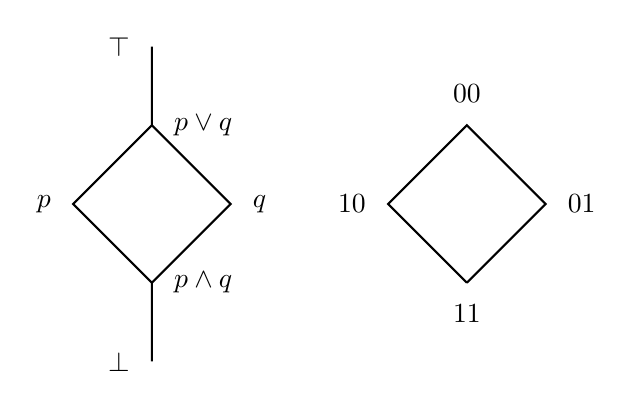
\begin{tikzpicture}[node distance=15pt, label distance=1pt]
      \pos{(0,-1)} %
     \pob{(0,0)} %
      \pob{(-1,1)} %
      \pob{(1,1)} %
      \pos{(0,2)} %
      \pob{(0,3)} %
       
      \draw[thick] (0,-1) -- (0,0) -- (-1,1) -- (0,2) -- (0,3);
      \draw[thick] (0,0) -- (1,1) -- (0,2);
  
      \node[label=left:{$\bot$}] at (0,-1) {};
      \node[label=right:{$p \wedge q$}] at (0,0) {};
      \node[label=left:{$p$}] at (-1,1)  {};
      \node[label=right:{$q$}] at (1,1) {};
      \node[label=right:{$p \vee q$}] at (0,2) {};
      \node[label=left:{$\top$}] at (0,3) {};
        
  
      \po{(4,0)} %
      \po{(3,1)} %
      \po{(5,1)} %
      \po{(4,2)} %
      \draw[thick] (4,0) -- (3,1) -- (4,2) -- (5,1) -- (4,0);
  
      \node[label=below:{11}] at (4,0) {};
      \node[label=left:{10}] at (3,1) {};
      \node[label=right:{01}] at (5,1) {};
      \node[label=above:{00}] at (4,2) {};
      \end{tikzpicture}
      \end{center}
      \caption{The free distributive lattice on two generators, and its dual poset.}
      \label{fig:freedltwo}
      \end{figure}
 
 In the figure on the right, we depict the dual poset as $(2,\preceq)^{\{p,q\}}$, i.e., the set of functions from $\{p,q\}$ to $2$, ordered pointwise, where the order on $2$ is given by $1\preceq 0$. The idea behind this is the following. As we know from Definition~\ref{def:Priestleydualspace}, we may choose to see the dual as $\Hom_\DL(F_{\DL}(\{p,q\}),\btwo)$ in the reverse point-wise order. Since $F_{\DL}(\{p,q\})$ is generated by $p$ and $q$, each such homomorphism is totally determined by its restriction to $\{p,q\}$. Also, by the universal property, \emph{every} function from $\{p,q\}$ to $2$ is the restriction of such a homomorphism.
 
  In the dual poset, we have denoted each function $f \colon \{p, q\} \to 2$ as a pair $f(p)f(q)$. For example, the element $p$ in the lattice corresponds to the down-set  $\{10, 11\}$ of the  dual poset while the element $\bot$ corresponds to the empty down-set, and the element $p \vee q$ corresponds to the down-set $\{10, 01, 11\}$.
 Thus, we see that the concrete incarnation of $F_{\DL}(\{p,q\})$ obtained via duality is given by the universal arrow 
\[
e\colon \{p,q\}\to \Down\left((2,\preceq)^{\{p,q\}}\right)\!, \ p\mapsto {\downarrow} \chi_{p},
\]
where $\chi_{p}$ is the characteristic function of the singleton $\{p\}$ and the order on $2$ is given by $1\preceq 0$.  
 
From a logic perspective, the elements of the dual poset correspond to lines in a truth table for propositional logic on two variables, and the subset associated to a formula $\phi$ is the set of lines in the truth table at which $\phi$ is true. This is precisely as conceived by logicians going back to Boole's fundamental work \cite{Boole1847}.

We here obtained the universal arrow $e$  as a map to the \emph{down}-sets of $2^{\{p,q\}}$ in the point-wise order relative to the ``upside down'' order on $2$, in which $1\preceq 0$. Note that this map may alternatively be described using \emph{up}-sets and the poset $\btwo$, which is $\{0,1\}$ with the usual order, in which $0\leq 1$, as the map
\[
\{p,q\}\to \Up\left(\btwo^{\{p,q\}}\right)\!,\  p\mapsto {\uparrow} \chi_{p}.
\]
These are two alternate descriptions of one and the same concrete incarnation of the free distributive lattice over the set $\{p,q\}$. Our reason for sticking with the ``upside down'' version of $2$ is that it morally is not the lattice $\btwo$, but the poset dual to $\bf 3$, the three element chain, see Exercise~\ref{exe:freeiscoproduct} in Chapter~\ref{ch:categories}.
  \end{example}
 We now proceed to make the corresponding argument for an arbitrary set $V$. %
For a set $V$, let $2^V$ denote the set of functions from $V$ to $2$. We will show (Proposition~\ref{prop:freeDL-duality}) that the dual space of $F_{\DL}(V)$ is order-homeomorphic to the following \emphind{ordered generalized Cantor space}. %

\begin{definition}\label{dfn:ordered-general-cantor}
Let $V$ be a set. We define the topology $\pi$ on $2^V$ to be the product topology, where $2$ carries the discrete topology. We define the partial order $\preceq$ on $2^V$, for $x, y \in 2^V$, by 
  \[ f \preceq g \iff \text{ for all } v \in V, \text{ if } g(v) = 1 \text{ then } f(v) = 1.\]
The ordered topological space $(2^V, \pi, \preceq)$ is called the \emphind{ordered generalized Cantor space} over $V$. The topological space $(2^V, \pi)$ is called \emphind{generalized Cantor space}, and $(2^\mathbb{N}, \pi)$ is the (classical) \emphind{Cantor space}.
\end{definition}

  Note that the topology $\pi$ on $2^V$ has as a subbasis the sets of the form
  \[ \sem{v \mapsto a} := \{ f \in 2^V \ \colon \ f(v) = a \},\]
  where $v$ ranges over the elements of $V$ and $a = 0,1$. 

  Note also that $\preceq$ is the pointwise order with respect to the order on $2$ in which $1 \leq 0$, as in Example~\ref{exa:twogen-logic} above; see Remark~\ref{rem:free-dl-as-upsets} below for an alternative description using up-sets and the order $\btwo$, in which $0 \leq 1$.%

  \begin{proposition}\label{prop:freeDL-duality}  
  Let $V$ be a set. The Priestley dual space of the free distributive lattice over $V$ is order-homeomorphic to the ordered generalized Cantor space over $V$, and the function $s \colon V \to \ClD(2^V)$, which sends $v \in V$ to the clopen down-set $s(v) := \sem{v \mapsto 1}$, is a universal arrow. 
  \end{proposition}
  
  Our proof here uses the algebraic fact, already proved above, that there exists a free distributive lattice over $V$. It is possible to give a proof ``from scratch'' that does not use this fact, see Exercise~\ref{exe:freeDL-dual-altproof}.
  \begin{proof}
  Let $e \colon V \to F$ be a free distributive lattice over $V$ and denote by $(X,\tau,\leq)$ the Priestley dual space of $F$. We will first exhibit an order-homeomorphism between $X$ and the ordered generalized Cantor space over $V$. Note that, for any point $x \in X$, the corresponding homomorphism $h_x \colon F \to \btwo$ must be of the form $\bar{f_x}$ for some function $f_x \colon V \to 2$: indeed, $h_x \colon F \to \btwo$ is equal to $\bar{f_x}$ for $f_x := h \circ e$. Let us write $\phi$ for the surjective function from $2^V$ to $X$ that sends $f \colon V \to 2$ to the element $x \in X$ with $h_x = \bar{f}$.%
  
  We now show that $\phi$ is an order-embedding, i.e., that for any functions $f, g \colon V \to 2$, we have $f \preceq g$ if, and only if, $\phi(f) \leq \phi(g)$ in $X$. First, if $\phi(f) \leq \phi(g)$ in $X$, then $\bar{f} \geq \bar{g}$ pointwise, so in particular $f = \bar{f} \circ e \geq \bar{g} \circ e = g$ pointwise, which means $f \preceq g$ by definition.
  For the other direction, note that, if $f \preceq g$, then the set $\{u \in F \ \colon \ \bar{f}(u) \geq \bar{g}(u)\}$ is a sublattice of $F$ containing $V$, and must therefore be equal to $F$ by Proposition~\ref{prop:free-generated}. It follows that $\phi$ is an order-isomorphism between the posets $(2^V, \preceq)$ and $(X,\leq)$.
  
  We now show that $\phi$ is a homeomorphism from $(2^V,\pi)$ to $(X,\tau)$. Note first that, by Proposition~\ref{prop:free-generated}, the set $e[V]$ generates $F$, so that the image of $e[V]$ under the isomorphism $\widehat{(-)} \colon F \to \ClD(X)$ also generates the topology on $X$ as a subbasis. To establish continuity of $\phi$, it therefore suffices to show that $\phi^{-1}(\widehat{e(v)})$ is open for every $v \in V$. Let $v \in V$ and $f \in 2^V$. We then have that $\phi(f) \in \widehat{e(v)}$ if, and only if, $\bar{f}(e(v)) = 1$, if, and only if, $f(v) = 1$. Thus, for any $v \in V$, we have 
  \begin{equation}\label{eq:phi-to-cylinder}
    \phi^{-1}(\widehat{e(v)}) = \sem{v \mapsto 1},
  \end{equation} 
 a clopen set in the product topology $\pi$. Since the sets $\sem{v \mapsto 1}$ and their complements form a subbasis for the clopen sets of the topology $\pi$, and $\phi$ is a bijection, we also immediately obtain from the equality (\ref{eq:phi-to-cylinder}) that $\phi$ is an open map. Finally, (\ref{eq:phi-to-cylinder}) shows that the diagram
 \begin{center}
   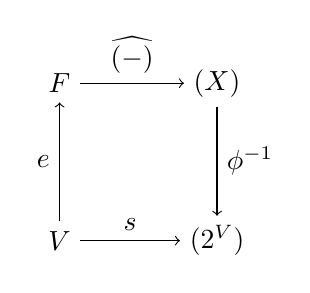
\begin{tikzpicture}
    \node (F) at (0,2) {$F$};
    \node (CLDX) at (2,2) {$\ClD(X)$};
     \node (V) at (0,0) {$V$};
    \node (CLD2V) at (2,0) {$\ClD(2^V)$};

    \draw[->] (V) to node[left] {$e$} (F);
    \draw[->] (F) to node[above] {$\widehat{(-)}$} (CLDX);
    \draw[->] (CLDX) to node[right] {$\phi^{-1}$} (CLD2V);
    \draw[->] (V) to node[above] {$s$} (CLD2V);
   \end{tikzpicture}
 \end{center}
 commutes, and therefore the function $s$ is a universal arrow, since the arrow $e$ is universal, $\phi^{-1} \circ \widehat{(-)}$ is an isomorphism, and isomorphisms preserve universal arrows (cf. Exercise~\ref{exe:universal-preserved-by-iso}).
  \end{proof}


  \begin{remark}\label{rem:free-dl-as-upsets}
    The alternative explanation of the free distributive lattice as up-sets instead of down-sets from Example~\ref{exa:twogen-logic} carries over to the general case. In particular, note that the function $s$ from Proposition~\ref{prop:freeDL-duality} may also be described as the function $s \colon V \to \ClU(\btwo^V)$ which sends $v$ to $\sem{v \mapsto 1}$, where now $\btwo$ is the order on $2$ in which $0 \leq 1$.

    A different kind of order symmetry in this context is the fact that the free distributive lattice is anti-isomorphic to itself. In terms of the concrete representation of the free distributive lattice as clopen down-sets of the ordered generalized Cantor space, we may consider the function $t \colon V \to \ClU(2^V)^\op$ that sends $v \in V$ to $t(v) := \sem{v\mapsto 0}$. Its unique lifting $\bar{t}$ along $s$ is an isomorphism from $\ClD(2^V)$ to $\ClU(2^V)^\op$, which may be described concretely by sending a clopen down-set $D$ to the clopen up-set $2^V \setminus D$.
  \end{remark}

  \begin{remark}
    We outline an alternative, more abstract proof of Proposition~\ref{prop:freeDL-duality}, by using some forward references to the categorical language that we will develop in Chapter~\ref{ch:categories}; see also Exercise~\ref{exe:freeiscoproduct}.  First, using the categorical fact that `left adjoints preserve colimits' (see Exercise~\ref{exe:left-ad-pres-colimits} in Chapter~\ref{ch:categories}), the free distributive lattice over a set $V$ must be the $V$-fold coproduct of the free distributive lattice over a singleton set. Now, the free distributive lattice on one generator $p$ is easily seen to be the three-element chain $\{ \bot < p < \top \}$, whose dual is $\{p, \top\}$. Using the fact that the category of Priestley spaces contains arbitrary products of finite posets (see Example~\ref{exa:priestley-as-profinite posets}), we may now recover Proposition~\ref{prop:freeDL-duality} directly from the categorical fact that a dual equivalence sends any coproduct of distributive lattices to a corresponding product of Priestley spaces.
  \end{remark}
  
  
  The \emphind{free Boolean algebra} over a set $V$ can be defined in an entirely analogous way to the free distributive lattice: it is a Boolean algebra $A$, together with a function $e \colon V \to A$, such that for every function $f \colon V \to B$ with $B$ a Boolean algebra, there exists a unique homomorphism $\bar{f} \colon A \to B$ such that $\bar{f} \colon e = f$. The proofs of Proposition~\ref{prop:free-unique}~and~\ref{prop:free-generated} can be carried out in the same way for the free Boolean algebra, as well as the algebraic construction of the free Boolean algebra: this is now the Lindenbaum-Tarski algebra of classical propositional logic. Alternatively, we may combine the free distributive lattice with the Boolean envelope\index{Boolean envelope} construction (cf. Section~\ref{sec:boolenv-duality}) to obtain the free Boolean algebra.
  \begin{lemma}\label{lem:freeDLplusboolenv}
    Let $V$ be a set. The Boolean envelope of the free distributive lattice over $L$ is the free Boolean algebra over $V$.
  \end{lemma}
  \begin{proof}
    Let $i \colon V \to F(V)$ be the free distributive lattice over $V$, and let $j \colon F(V) \to F(V)^-$ be the Boolean envelope. We claim that $e := j \circ i \colon V \to F(V)^-$ has the required universal property for the free Boolean algebra. Indeed, for any function $f \colon V \to B$ with $B$ a Boolean algebra, there is first, by definition of the free distributive lattice, a unique lattice homomorphism $\bar{f} \colon F(V) \to B$ with $\bar{f} \circ i = f$, and then, by definition of the Boolean envelope, a unique homomorphism $\bar{f}^- \colon F(V)^- \to B$ such that $\bar{f}^- \circ j = \bar{f}$. Now $\bar{f}^- \circ e = \bar{f}^- \circ j \circ i = \bar{f} \circ i = f$; the uniqueness of $\bar{f}^-$ is clear from the uniqueness parts of the universal properties of the free distributive lattice and the Boolean envelope.
  \end{proof}
  \begin{corollary}\label{cor:freeBA-duality}
  Let $V$ be a set. The Boolean algebra of clopen sets of the generalized Cantor space, $(2^V, \pi)$, is the free Boolean algebra over $V$ via the function $s$ which sends any $v \in V$ to the clopen set $\sem{v \mapsto 1}$.
  \end{corollary}
  \begin{proof}
    Combine Proposition~\ref{prop:boolenv}, Proposition~\ref{prop:freeDL-duality}, and Lemma~\ref{lem:freeDLplusboolenv}.
  \end{proof}
In case $V$ is countable, the free Boolean algebra over $V$ is countable, and  it is \emphind{atomless}, i.e., it does not have any atoms. In fact, one may use model-theoretic techniques to prove that this is the \emph{unique}, up to isomorphism, countable and atomless Boolean algebra, and it is a central structure in several parts of logic. Its dual is the classical Cantor space $2^\N$.
\exercises

\exercise\label{exe:universal-preserved-by-iso}
Let $V$ be a set, and suppose that $e \colon V \to F$, $e' \colon V \to F'$ are functions to distributive lattices $F$ and $F'$, and $\phi \colon F' \to F$ is a lattice isomorphism. Prove that $e$ is a universal arrow if, and only if, $e'$ is a universal arrow.

\exercise\label{exe:freeBA-on-2}
How many elements does the free Boolean algebra on two generators have? Draw its Hasse diagram, labeling each of its elements with a corresponding Boolean algebra term.


\begin{exercise}\label{exe:freeDL-algebraic}
  This exercise asks you to supply some details in the proof of Proposition~\ref{prop:freeDL-algebraic}.
  \begin{enumerate}
    \item Show that $\equiv$ is congruential on $T(V)$.
    \item Show that $T(V)/{\equiv}$, with operations defined as in the paragraph before Proposition~\ref{prop:freeDL-algebraic}, satisfies all the defining equations of a distributive lattice. \hint{This is almost immediate from the definition of $\equiv$.
    \item Prove in detail that the function $\bar{f}$ defined in the proof of Proposition~\ref{prop:freeDL-algebraic} is a homomorphism and that $\bar{f} \circ e = f$.}
    \item Prove that if $g \colon T(V)/{\equiv} \to L$ is a homomorphism and $g \circ e = f$, then $g = \bar{f}$.
  \end{enumerate}
\end{exercise}

\begin{exercise}\label{exe:Vto2}
Let $V$ be a set and $L$ a distributive lattice. Show that the poset $L^V$ of all functions from $V$ to $L$ with the pointwise order is order isomorphic to the poset of all homomorphisms from $F_{\DL}(V)$ to $L$ also with the pointwise order.
\end{exercise}

\begin{exercise}\label{exe:freeDL-dual-altproof}
  This exercise outlines a proof of Proposition~\ref{prop:freeDL-duality} that does not rely on generalities from universal algebra, and gives a more concrete construction of the lifting homomorphisms. %
  Let $V$ be a set, and $(2^V, \preceq, \pi)$ the ordered generalized Cantor space over $V$. %

  \begin{enumerate}
    \item Prove that, for each $v \in V$, the set $s(v) := \sem{v \mapsto 1}$ is a clopen down-set in $(2^V, \preceq, \pi)$.
    \item Let $K$ be a clopen down-set of $(2^V, \preceq, \pi)$. Prove, using the compactness of $2^V$ and the definition of the order, that there exists a finite collection $\mathcal{C}$ of finite subsets of $V$ such that $K = \bigcup_{C \in \mathcal{C}} \bigcap_{v \in C} s(v)$.
    \item Give a direct proof that, for any function $h \colon V \to L$, with $L$ a distributive lattice, there exists a unique homomorphism $\bar{h} \colon \ClD(2^V) \to L$ such that $\bar{h} \circ s = f$.
  \end{enumerate}
\end{exercise}

\section{Quotients and subs}\label{sec:quotients-and-subs}
In many applications of Priestley duality, including some in the later chapters of this book, we use the dual space of a lattice to study its quotient lattices and sublattices, or we use the dual lattice of a space to study its quotient spaces and subspaces. 
In this section, we exhibit two Galois connections, between relations and subsets, which in particular allow us to prove that (i) the quotients of a distributive lattice are in an order-reversing bijection with the closed subspaces of its Priestley dual space; and (ii) the sublattices of a distributive lattice are in an order-reversing bijection with the Priestley quotients of its Priestley dual space. While (i) and (ii) can also be deduced in a more abstract way from Theorem~\ref{thm:priestleyduality} using category theory (see Theorem~\ref{thm:subquotient-duality-categorically}), the Galois connections that we develop in this chapter do a bit more. In concrete applications, these Galois connections are what allow us to define so-called \emphind{equations} on either side of the duality.

Let $L$ be a distributive lattice with Priestley dual space $X$. We will first show how to associate a closed subspace $\sem{R}$ to any binary relation $R$ on $L$. Here, a pair that is in such a relation is thought of as an equation, since it acts as a constraint on the other side of the duality. This motivates us to write, in this section only, pairs of elements with the notation $a \approx b$, instead of $(a,b)$; note that this is only a notation, ``$a \approx b$'' denotes nothing more than ``the pair $(a,b)$''. 

For any pair of elements $a \approx b \in L^2$, we define a clopen subset $\sem{a \approx b}$ of  $X$ by $$\sem{a \approx b} := (\widehat{a} \cap \widehat{b}) \cup (\widehat{a}^c \cap \widehat{b}^c) = \{x \in X \ | \ x \in \widehat{a} \text{ iff } x \in \widehat{b} \}.$$
We extend this assignment to any binary relation $R$ on $L$, by defining
$$\sem{R} := \bigcap_{a \approx b \in R} \sem{a \approx b} = \{x \in X \ | \ \text{ for every } a \approx b \text{ in } R,\; x \in \widehat{a} \text{ iff } x \in \widehat{b} \}.$$
Conversely, for any element $x \in X$, we define a binary relation $\theta(x)$ on $L$ by
$$\theta(x) := \ker(h_x) = (F_x \times F_x) \cup (I_x \times I_x) = \{a \approx b \ | \ x \in \widehat{a} \text{ iff } x \in \widehat{b}\}.$$
We extend this assignment to subsets $S \subseteq X$ by defining
$$\theta(S) := \bigcap_{x \in S} \theta(x) = \{a \approx b \ | \ \widehat{a} \cap S = \widehat{b} \cap S\}.$$
Note that the above definitions of $\sem{-}$ and $\theta$ are a special case of the functions $u$ and $\ell$ introduced in Example~\ref{exa:galoisconnection}, if we consider the relation $\mathcal{R} \subseteq L^2 \times X$ given by $(a \approx b, x) \in \mathcal{R}$ iff $x \in \sem{a \approx b}$.
\begin{proposition}\label{prop:quotientlattice-subspace}
  Let $L$ be a distributive lattice with dual Priestley space $X$.  The two functions $\sem{-} \colon \mathcal{P}(L^2) \leftrightarrows \mathcal{P}(X)^\op \colon \theta$ form an adjunction, whose fixed points on the left are the lattice congruences on $L$, and whose fixed points on the right are the closed subspaces of $X$.



\end{proposition}
\begin{proof}
  It is clear from the definitions that both $\sem{-}$ and $\theta$ are order-reversing. Moreover, for any $a \approx b \in L^2$ and $x \in X$, we have that $x \in \sem{a \approx b}$ if, and only if, $\theta(x) \ni a \approx b$. It now easily follows from the definitions that for any $R \subseteq L^2$ and $S \subseteq X$, we have $S \subseteq \sem{R}$ if, and only if, $ \theta(S) \supseteq R$. Thus, $\sem{-}$ and $\theta$ are a contravariant adjunction between binary relations on $L$ and subsets of $X$.

For the statement about fixed points, we need to show that the image of $\sem{-}$ consists of the closed subsets of $X$, and that the image of $\theta$ consists of the congruences on $L$. First, since each $\sem{a \approx b}$ is clopen, $\sem{R}$ is closed for every binary relation $R$. Conversely, let $C \subseteq X$ be any closed set. We show that $C = \sem{\theta(C)}$.  By adjunction, we have $C \subseteq \sem{\theta(C)}$. We prove the other inclusion by contraposition. Let $x \not\in C$ be arbitrary. Using the basis for the Priestley topology given in Lemma~\ref{lem:Priestleybasis}, pick $a, b \in L$ such that $x \in \widehat{a} \setminus \widehat{b}$ and $C$ is disjoint from $\widehat{a} \setminus \widehat{b}$. Note that the latter implies that $a \approx a \wedge b$ in $\theta(C)$, since for any $y \in C$, we have $y \in \widehat{a}$ if, and only if, $y \in \widehat{a} \cap \widehat{b}$. However, $x \in \widehat{a}$ but $x \not\in \widehat{a \wedge b}$, so $x \not\in \sem{\theta(C)}$, as required.

We now show that the image of $\theta$ consists of the congruences on $L$. Note that $\theta(S)$ is a congruence for any $S$, as it is an intersection of congruences. Let $\phi$ be a congruence on $L$. We show that $\phi = \theta(\sem{\phi})$. The left-to-right inclusion holds by adjunction. For the other direction, we reason by contraposition, and assume $(a,b) \not\in \phi$. Denote by $p \colon L \onto L/{\phi}$ the lattice quotient by the congruence $\phi$. Then $p(a) \neq p(b)$, and we assume without loss of generality that $p(a) \nleq p(b)$. By Theorem~\ref{thm:DPF} applied to $L/{\phi}$, the filter ${\uparrow}p(a)$ and the ideal ${\downarrow}p(b)$, pick a prime filter $G$ in $L/{\phi}$ containing $p(a)$ but not $p(b)$. The inverse image under the homomorphism $p$, $F_x := p^{-1}(G)$, is a prime filter of $L$ which contains $a$ but not $b$. Moreover, for any $(c,d) \in \phi$, we have $c \in F_x$ if, and only if, $p(c) \in G$, if, and only if, $d \in F_x$, since $p(c) = p(d)$ by assumption. Thus, $x \in \sem{\phi}$, and we conclude that $(a,b) \not\in \theta(\sem{\phi})$.
\end{proof}

From Proposition~\ref{prop:quotientlattice-subspace}, we deduce the following theorem, which shows how to explicitly compute the subspace dual to a lattice quotient generated by some equations.
\begin{theorem}
Let $L$ be a distributive lattice with dual Priestley space $X$, and let $R$ be a binary relation on $L$. Then the lattice congruence generated by $R$, $\gen{R}$, is equal to $\theta(\sem{R})$, and the Priestley dual space of $L/\gen{R}$ is order-homeomorphic to the closed subspace $\sem{R}$ of $X$.
\end{theorem}
\begin{proof}
In general, for any adjunction $f \colon P \leftrightarrows Q \colon g$, for any $p \in P$, $gf(p)$ is the minimum of $\mathrm{im}(g) \cap {\uparrow}p$ (Exercise~\ref{exe:adjunctions}.\ref{itm:minimumimage} in Chapter~\ref{ch:order}). In particular, using that $\mathrm{im}(\theta)$ consists of the congruences on $L$, $\theta(\sem{R})$ is the smallest congruence containing $R$. Let $Y$ denote the Priestley dual space of the quotient lattice $L / \gen{R}$. The dual of the quotient map $p \colon L \onto L / \gen{R}$ is the continuous order-preserving function $i \colon Y \to X$ which can be defined by $h_{i(y)} := h_y \circ p$, for every $y \in Y$. Note that $i$ is an order embedding: if $y \nleq y'$ in $Y$, then there exists $b \in L / \gen{R}$ such that $y \in \widehat{b}$ and $y' \not\in \widehat{b}$, and since $p$ is surjective, pick $a \in L$ such that $b = p(a)$. Then $i(y) \in \widehat{a}$ and $i(y') \not\in \widehat{a}$, so $i(y) \nleq i(y')$. Finally, for any $x \in X$, we have that $x \in \sem{\gen{R}}$ if, and only if, $\gen{R} \subseteq \theta(\{x\}) = \ker(h_x)$, using the Galois connection between $\sem{-}$ and $\theta$. The latter holds if, and only if, $h_x = h_y \circ p$ for some $y \in Y$. Therefore, the image of $i$ is equal to $\sem{\gen{R}} = \sem{\theta(\sem{R})} = \sem{R}$, using the general fact that $gfg = g$ for any adjunction $(f,g)$ (see again Exercise~\ref{exe:adjunctions}). Thus, $i$ is a homeomorphism between $Y$ and the closed subspace $\sem{R}$, as required.
\end{proof}

A second theorem mirrors the previous one, but on the space side.
\begin{theorem}\label{thm:closure-via-duality}
Let $X$ be a Priestley space with dual distributive lattice $L$, and let $S$ be a subset of $X$. Then the closure of $S$, $\overline{S}$, is equal to $\sem{\theta(S)}$, and the lattice dual to $\overline{S}$ is isomorphic to the quotient $L/\theta(S)$.
\end{theorem}
\begin{proof}
Left as Exercise~\ref{exe:closure-via-duality}.
\end{proof}

\begin{remark}
What is interesting about Proposition~\ref{prop:quotientlattice-subspace} is that we can start, on either side of the duality, with an unstructured set: an arbitrary subset $R\subseteq L\times L$ or $S\subseteq X$ and, by applying the Galois connection, we end up with only the structured subsets: that is, $\sem{R}$ is not just a subset of $X$, but it is a Priestey subspace of $X$ and $\theta(S)$ is not just a subset of $L\times L$ but it is a congruence of $L$.
\end{remark}

We give a few simple examples. The reader is asked to supply the details in Exercise~\ref{exe:quot-subspace}.

\begin{example}\label{exa:quot-subspace1}
Let $B$ be the eight element Boolean algebra. 
\begin{figure}[htp]
\begin{center}
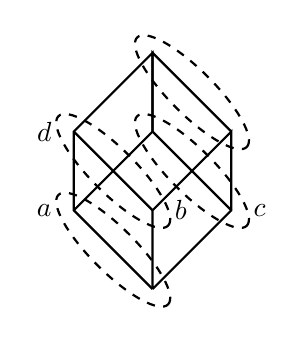
\begin{tikzpicture}[node distance=15pt, label distance=1pt]
  \po{(0,-1)} 

  \po{(-1,0)}
  \po{(1,0)}
  \po{(0,0)}

  \po{(-1,1)}
  \po{(0,1)}
  \po{(1,1)} 

  \po{(0,2)}
  
   
  \draw[thick] (0,-1) -- (-1,0) -- (-1,1) -- (0,2) -- (0,1) -- (-1,0);
  \draw[thick] (0, -1) -- (0, 0) -- (1,1) -- ((1, 0) -- (0,-1); 
  \draw[thick] (1,0) -- (0,1) -- (0, 2) -- (1,1);
  \draw[thick] (0,0) -- (-1,1);

  \node[label=left:{$a$}] at (-1,0) {};
  \node[label=left:{$d$}] at (-1,1) {};
  \node[label=right:{$b$}] at (0,0)  {};
  \node[label=right:{$c$}] at (1,0) {};

  \draw[thick, dashed, rotate around={315:(-.5,-.5)}] (-.5,-.5) ellipse (28pt and 8pt);
  \draw[thick, dashed, rotate around={315:(-.5,.5)}] (-.5,.5) ellipse (28pt and 8pt);
  \draw[thick, dashed, rotate around={315:(.5,.5)}] (.5,.5) ellipse (28pt and 8pt);
  \draw[thick, dashed, rotate around={315:(.5,1.5)}] (.5,1.5) ellipse (28pt and 8pt);
\end{tikzpicture}
\end{center}
\caption{A congruence on the eight element Boolean algebra}
\label{fig:quot-subspace1}
\end{figure}
Its dual space is $X=\{x,y,z\}$, where $F_x={\downarrow}a$, $F_y={\downarrow}b$, and $F_z={\downarrow}c$. The equation $b\approx d$ corresponds to the subspace $S=\{y,z\}$ and the corresponding congruence is as depicted in Figure~\ref{fig:quot-subspace1}.
\end{example}

\begin{example}\label{exa:quot-subspace2}
Let $X$ be the poset depicted on the left in Figure~\ref{fig:quot-subspace2} and let $S=\{x,y\}$.
\begin{figure}[htp]
  \begin{center}
  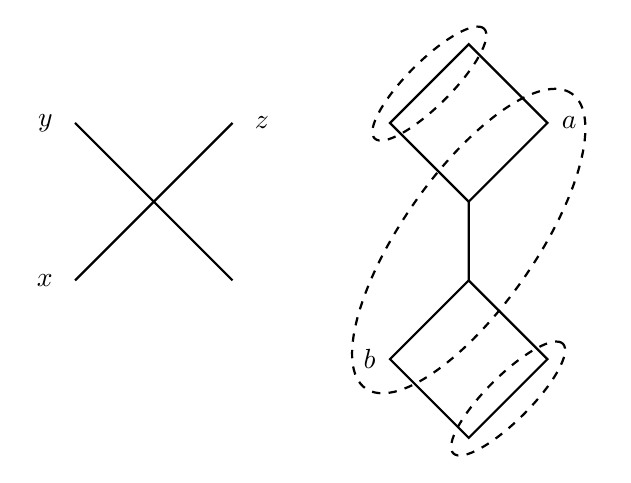
\begin{tikzpicture}[node distance=15pt, label distance=1pt]
    \po{(-1,-1)}
    \po{(1,-1)}
    \po{(0,0)}
    \po{(-1,1)}
    \po{(1,1)}
    
     
    \draw[thick] (-1,-1)--(0,0)--(-1,1);
    \draw[thick] (1,-1)--(0,0)--(1,1); 
    \node[label=left:{$x$}] at (-1,-1) {};
    \node[label=left:{$y$}] at (-1,1) {};
    \node[label=right:{$z$}] at (1,1)  {};
    \node[label=right:{$a$}] at (4.9,1) {};
    \node[label=left:{$b$}] at (3.1,-2) {};
    \po{(4,0)}
    \po{(3,1)}
    \po{(5,1)}
    \po{(4,2)}

    \po{(4,-1)}
    \po{(3,-2)}
    \po{(5,-2)}
    \po{(4,-3)}

    \draw[thick] (4,0)--(3,1)--(4,2)--(5,1)--(4,0);
    \draw[thick] (4,0)--(4,-1)--(3,-2)--(4,-3)--(5,-2)--(4,-1);
    
    \draw[thick, dashed, rotate around={45:(3.5,1.5)}] (3.5,1.5) ellipse (28pt and 8pt);
    \draw[thick, dashed, rotate around={45:(4.5,-2.5)}] (4.5,-2.5) ellipse (28pt and 8pt);
    \draw[thick, dashed, rotate around={55:(4,-0.5)}] (4,-0.5) ellipse (65pt and 24pt);

  \end{tikzpicture}
  \end{center}
  \caption{A poset, its down-set lattice, and the congruence corresponding to the subset $\{x,y\}$.  Here, $a$ corresponds to the downset ${\downarrow}z$ and $b$ corresponds to the downset $\{x\}$.} 
  \label{fig:quot-subspace2}
  \end{figure}
The dual lattice and the congruence corresponding to $S$ are as depicted on the right in the same figure. Furthermore, the subspace $S$ is given by the equation $a\approx b$.
\end{example}

\begin{example} \label{exa:remainderofbetaX}
Recall the Stone-{\v C}ech compactification $\beta X$ of a set $X$, introduced in  Example~\ref{exa:StoneCechcompactification}. As remarked in Example~\ref{exa:StoneCechcompactification}, every point of $X$ is isolated in $\beta X$, so that $X$ is an \emph{open} subspace of $\beta X$. The closed set ${}^*X := \beta X\setminus X$ is known as the \emphind{remainder} of the Stone-{\v C}ech compactification $\beta X$. Since it is a closed subspace of the dual space of $\mathcal{P}(X)$, it corresponds to a quotient of the Boolean algebra $\mathcal{P}(X)$. 
This quotient is given by the set of equations $\{x\} \approx \emptyset$ on $\cP(X)$, where $x$ ranges over the elements of $X$.
Indeed, using an argument like the one in Example~\ref{exa:fincofsubsetsdual}, one may prove that, for any $\mu \in \beta X$, we have that $\mu \in X$ if, and only if, $\mu$ contains a finite set. It follows that in the congruence dual to ${}^*X$, the equivalence class of $\emptyset$, is the collection of finite sets. As in any Boolean algebra, the entire congruence is now determined by the class of the bottom element: two sets $v$ and $v'$ will be related by the congruence if, and only if, their symmetric difference is finite.
This Boolean algebra is often denoted $\mathcal{P}(X)/\mathrm{fin}$, and is well studied in set theory and general topology.
\end{example}

\subsection*{Sublattices and Priestley quotient spaces}
A very similar story to the one above can be told for sublattices and quotients of Priestley spaces that are themselves Priestley spaces. In fact, the ensuing notion of Priestley space (in)equations is a very important tool in the theory of automata and regular languages, as we will see in Chapter~\ref{ch:AutThry}.

We give the necessary definitions and statements of the relevant theorems, and we note that in fact the lattice-quotient--closed-subspace duality from the previous subsection and the sublattice--Priestley-quotient-space duality are, in a sense, dual to each other.

We first introduce the notion of \emph{quotient space} in the context of Priestley spaces. This is an instance of a more general notion of quotient of ordered topological spaces, but we only need it in this setting.
\begin{definition}\label{def:compatible}
A preorder $\preceq$ on a Priestley space $(X, \leq_X, \tau)$ is \emph{compatible} if, for any $x, y \in X$, if $x \not\preceq y$, then there exists a $\tau$-clopen $\preceq$-down-set $K$ in $X$ such that $x \in K$ and $y \not\in K$.
\end{definition}
Compatible preorders on $X$ give an intrinsic description of the Priestley spaces $Y$ which are quotients of $X$, i.e., for which there exists a continuous order-preserving surjective map $X \onto Y$. We just indicate here what this means, and ask you to fill in the details in the exercises. First, for any $p \colon X \onto Y$, the preorder on $X$ defined by $x \preceq x'$ iff $p(x) \leq_Y p(x')$ is compatible (see Exercise~\ref{exe:compatible-from-quotient}). Conversely (see Exercise~\ref{exe:compatible-to-quotient}), if $\preceq$ is a compatible preorder on $X$, denote by $Y$ the poset reflection of the preordered set $(X,\preceq)$. That is, as a set,  $Y$ is $X/\equiv$ where ${\equiv} := {\preceq \cap \succeq}$, and write $q \colon X \onto Y$ for the quotient map. Then the partial order $\leq_Y$ on the poset reflection is defined, for any $y = q(x)$ and $y' = q(x')$ in $Y$, by $y \leq_Y y'$ iff $x \preceq x'$. The \emph{quotient topology} on $Y$ is defined by $\tau_Y := \{U \subseteq Y \ \mid \ q^{-1}(U) \in \tau_X\}$. The ordered topological space $(Y, \leq_Y, \tau_Y)$ is a Priestley space, and the function $q$ is a continuous order-preserving map. Moreover, any continuous map $f \colon X \to Z$, with $Z$ a Priestley space and $x \preceq y$ implies $f(x) \leq_Z f(y)$, factors uniquely through $p$. We will say that $(Y, \leq_Y, \tau_Y)$ is the quotient of the Priestley space $X$ by $\preceq$ and will denote it by $X/{\preceq}$.

Now let $L$ be a distributive lattice with dual Priestley space $X$. For any element $a \in L$,  we define a binary relation $\preceq_a$ on $X$ by
\[ x \preceq_a y \iff y \in \widehat{a} \text{ implies } x \in \widehat{a},\]
i.e., ${\preceq_a} := \widehat{a} \times (X \setminus \widehat{a})$, which is a clopen down-set in the Priestley space $X \times X^\op$. For any subset $A \subseteq L$, we define ${\preceq_{A}} := \bigcap_{a \in A} {\preceq_a}$, i.e.,
\[ x \preceq_A y \iff \text{ for all } a \in A, \text{ if } y \in \widehat{a} \text{ then } x \in \widehat{a}.\]
Clearly, $\preceq_A$ is a preorder which contains the Priestley order $\leq$. We will see below that it is a compatible preorder, and that every compatible preorder is of this form.%

\begin{example}\label{exa:Priestley order as a compatible order}
Consider a Priestley space $(X,\leq, \tau)$ with dual lattice $L$. Notice (see Exercise~\ref{exe:Booleanspace}) that then $(X,=,\tau)$ is also a Priestley space. In fact, the dual lattice of this Priestley space is the Boolean algebra $L^-$ of all clopen subsets of $X$, also known as the Boolean envelope of $L$, see Corollary~\ref{cor:doubledualBA}. Of course, $L$ is a sublattice of $B$. The dual of the inclusion of $L$ into $L^-$ is simply the identity map on $X$, viewed as a continuous order-preserving map $\id_X\colon (X,=,\tau)\to(X,\leq, \tau)$. The corresponding compatible preorder is the partial order $\leq$ of $(X,\leq, \tau)$.

More generally, any injective homomorphism $i \colon L \into B$, with $B$ a Boolean algebra, factors as the composition of $e \colon L \into L^-$ and $\bar{i} \colon L^- \into B$. Dually, denoting by $(Y,\pi)$ the Boolean space dual to $B$, this gives a quotient map of Boolean spaces $f \colon (Y,\pi) \to (X,\tau)$, followed by $\id_X \colon (X, =, \tau) \to (X, \leq,\tau)$. This shows that sublattices of Boolean algebras can be understood dually by a Boolean equivalence relation together with a Priestley order on the quotient.
\end{example}

As before, the correspondence between compatible preorders and sublattices allows us to view pairs of elements $(x,y)$ from $X$ as constraints on $L$ yielding sublattices. However, as Example~\ref{exa:Priestley order as a compatible order} already shows, equating elements of the space is not a fine enough notion to witness all sublattices and we will need to think of pairs $(x,y)$ as \emph{inequations}. For this reason, we will denote pairs in $X\times X$ as $x\preceq y$ when we view them as constraints on the dual.

\begin{definition}\label{def:ineq}
For any pair $x\preceq y$ in $X^2$, we define the subset $\sem{x\preceq y}$ of $L$ by
\[ \sem{x\preceq y} := I_y \cup F_x = \{a \in L \ \mid \ \text{ if } y \in \widehat{a}, \text{ then } x \in \widehat{a} \}.\]
We will also write ``$a\ \models\ x\preceq y$'' to mean that $a \in \sem{x \preceq y}$, and we will say that $a$ \emphind{satisfies the inequation} $x\preceq y$.
For any relation $E$ on $X$, we define the subset $\sem{E}$ of $L$ by
\[ 
\sem{E} := \bigcap_{x\preceq y \in E} \sem{x\preceq y} = \{a \in L \, \mid \, \text{ for all } x\preceq y \in E, \ a\ \models\ x\preceq y \}.
\]
\end{definition}
\begin{proposition}\label{prop:sublattice-quotientspace}
  Let $L$ be a distributive lattice with dual Priestley space $X$.  The two functions $\preceq_{-} \colon \mathcal{P}(L) \leftrightarrows \mathcal{P}(X^2)^\op \colon \sem{-}$ form an adjunction, whose fixed points on the left are the sublattices of $L$, and whose fixed points on the right are the compatible preorders on $X$.
\end{proposition}
\begin{proof}
See Exercise~\ref{exe:sublattice-quotient-adjunction}.
\end{proof}

\begin{theorem}\label{thrm:sublatices-inequations}
  Let $L$ be a distributive lattice with dual Priestley space $X$.
  \begin{enumerate}
  \item For any subset $A$ of $L$, the sublattice generated by $A$ is equal to $\sem{\preceq_A}$, and the Priestley dual space of this sublattice is order-homeomorphic to the Priestley quotient $X/{\preceq_A }$.
  \item For any binary relation $E$ on $X$, the smallest compatible preorder containing $E$ is equal to $\preceq_{\sem{E}}$, and the lattice dual to the Priestley quotient by this preorder is isomorphic to $\sem{E}$.
  \end{enumerate}
\end{theorem}

\begin{remark}\label{rem:inequations}
One problem with compatible preorders, which has sometimes hampered their successful application, is that it is difficult to understand intrinsically in a Priestley space how to obtain the compatible preorder generated by a binary relation on the space. The existence of the Galois connection of Proposition~\ref{prop:sublattice-quotientspace} frees us from this problem and allows us to specify sublattices from arbitrary sets $E$ of inequality constraints of the form $x\preceq y$. 

This is similar to the fact that, in logic, we do not need to identify the full theory of a class of structures that we are interested in, since we may be able to capture it by a much smaller set of axioms.
\end{remark}

As mentioned above, we will see dual space (in)equations in action in Chapter~\ref{ch:AutThry}. In the meantime, we give two elementary examples.

\begin{example}[Sublattices of the free distributive lattice]\label{exa:sub-of-free}
Coming back to the example of the free distributive lattice on two generators, Example~\ref{exa:twogen-logic}, consider the sublattices $L_1 = \{\bot, p, \top\}$ and $L_2 = \{\bot, p \vee q, \top\}$. One may prove from the definitions that the corresponding quotients of $2^{\{p,q\}}$ are given by the equivalence relations $\equiv_1$ and $\equiv_2$, where $\equiv_1$ has classes $\{00, 01\}$ and $\{10,11\}$, while $\equiv_2$ has classes $\{00\}$ and $\{01,10,11\}$. We leave it as Exercise~\ref{exe:subs-of-freedl-two} to classify the other sublattices of this lattice.
\end{example}

\begin{example}[Equations for a subalgebra]\label{exa:equationssubalg}
In this example we will see how we can use extraneous structure on a dual space and lattice to identify a smaller set of equations for a subalgebra of an infinite Boolean algebra; this technique is further exploited in Chapter~\ref{ch:AutThry}. %

Consider the set $\bZ$ of integers, denote by $\bZ^+$ the subset of positive integers and by $\bZ^-$ the subset of negative integers; so $\bZ = \bZ^- \cup \{0\} \cup \bZ^+$. Let $M$ be the Boolean subalgebra of $\cP(\bZ)$ consisting of all those subsets $S$ of $\bZ$ such that \emph{both} $S\cap\bZ^+$ is either finite or co-finite, \emph{and} $S\cap\bZ^-$ is either finite or co-finite. One may then show (see Exercise~\ref{exe:equationssubalg}) that the dual space of $M$ is the `two-point compactification of $\bZ$' 
\[
\bZ_{-\infty}^{+\infty}=\bZ\cup\{-\infty,+\infty\},
\]
 which topologically is the disjoint union of the one-point compactification $\bZ^+\cup\{+\infty\}$ of $\bZ^+$ with the discrete topology and the one-point compactification $(\bZ\setminus\bZ^+)\cup\{-\infty\}$ of $\bZ \setminus \bZ^+$ with the discrete topology. (For the one-point compactification, see Example~\ref{exa:fincofsubsetsdual} and Exercise~\ref{exe:fincofsubsetsspace}.) Note in particular that any ultrafilter of $\cP(\bZ)$ is either principal, or contains exactly one of $\bZ^+$ or $\bZ \setminus \bZ^+$, using arguments similar to the ones in Example~\ref{exa:fincofsubsetsdual}. The dual of the inclusion $M\hookrightarrow\cP(\bZ)$ is the surjective function
\begin{align*}
\beta(\bZ)&\onto \bZ_{-\infty}^{+\infty}, \\
\mu&\mapsto\left\{ 
   \begin{array}{lll}
   k & \text{ if } & \{k\}\in\mu \text{ for some } k \in \bZ,\\
   +\infty & \text{ if } & \bZ^+\in\mu,\\%\in\beta(\bZ){\setminus}\bZ,\\
   -\infty & \text{ if } & \bZ \setminus \bZ^+\in\mu.%
   \end{array}
   \right.
\end{align*}
Thus, the compatible preorder on $\beta\bZ$ corresponding to the subalgebra $M$ of $\cP(\bZ)$ is the equivalence relation in which each $k\in \bZ$ is only related to itself, and two free ultrafilters $\mu$ and $\nu$ are related provided they either both contain $\bZ^+$, or both contain $\bZ \setminus \bZ^+$. 
That is, the remainder is split into two uncountable equivalence classes and each free ultrafilter is related to uncountably many other free ultrafilters.

By contrast, we will now show that, by using the successor structure on $\bZ$, the subalgebra $M$ can be `axiomatized' by a much `thinner' set of equations. For $\mu \in \beta\bZ$, write 
\[
\mu+1:=\{S\in\cP(\bZ)\mid S-1\in\mu\}=\{S+1\mid S\in\mu\},
\]
defining the continuous extension of the successor function on $\bZ$ to $\beta\bZ$, which is  the Priestley dual of the homomorphism $S\mapsto S-1$ on $\cP(\bZ)$. 
To describe the equational basis for $M$, for convenience, we abbreviate by $\mu+1 \approx \mu$ the conjunction of the two inequations $\mu+1 \preceq \mu$ and $\mu \preceq \mu+1$. Now consider the set of equations 
\begin{equation}\label{eq:equational-basis-twopoint}
\{\mu+1\approx\mu \mid \mu\in{}^*\bZ\},
\end{equation}
where we recall that ${}^*\bZ := \beta(\bZ) \setminus \bZ$, the \emph{remainder} of $\beta(\bZ)$, see Example~\ref{exa:remainderofbetaX}. 
We will show that the sublattice $M$ contains exactly those $S \in \cP(\bZ)$ that satisfy all the equations in (\ref{eq:equational-basis-twopoint}). 

To this end, note first that, for $S \in \cP(\bZ)$, $S$ satisfies $\mu+1 \approx \mu$ if, and only if, both $\mu$ and $\mu + 1$ contain $S$, or neither $\mu$ nor $\mu + 1$ contains $S$.
Now let $\mu$ be a free ultrafilter of $\cP(\bZ)$ and let $S\in M$. We show that $S\models \mu+1\approx\mu$. Since $\mu$ is prime and $\bZ^+\cup (\bZ \setminus \bZ^+)=\bZ\in\mu,$ it follows that either $\bZ^+\in\mu$ or $\bZ \setminus \bZ^+ \in\mu$. We treat the case $\bZ^+\in\mu$ and leave the other as an exercise. Now, if $S\cap\bZ^+$ is finite then, as $\mu$ is free, $S\not\in\mu$. Also $S\cap\bZ^+$ finite implies that $(S-1)\cap\bZ^+$ is finite and thus $S-1\not\in\mu$. So $S\models \mu+1\approx\mu$. If on the other hand $S\cap\bZ^+$ is co-finite, then, as 
$
(\bZ^+\setminus S) \cup (S\cap\bZ^+)=\bZ^+\in\mu, 
$
and $\mu$ is free, it follows that $S\cap\bZ^+\in\mu$. Furthermore, $S\cap\bZ^+$ co-finite implies that $(S-1)\cap\bZ^+$ is also co-finite and by the same argument we have $S-1\in\mu$ so that $S\models \mu+1\approx\mu$. This shows that
\[
M\subseteq\sem{\,\mu+1\approx\mu\mid \mu\in{}^*\bZ\,}.
\]
For the converse, suppose $S\not\in M$. Then $S\cap\bZ^+$ is neither finite or co-finite, or $S\cap\bZ^-$ is neither finite or co-finite. Again, we treat the first case and leave the second as an exercise. If $S\cap\bZ^+$ is neither finite or co-finite it follows that there is an infinite set $T\subseteq\bZ^+$ such that, for each $k\in T$
\[
k\not\in S \quad\text{ but }\quad k+1\in S.
\]
By the Prime Filter-Ideal Theorem~\ref{thm:DPF}, here applied to the Boolean algebra $\cP(\bZ)$, pick an ultrafilter  $\mu$ of $\cP(\bZ)$ which contains the filter ${\uparrow}T$ and is disjoint from the ideal $I$ consisting of all finite subsets of $\cP(\bZ)$. Since $\mu$ is disjoint from $I$, it is free, and since ${\uparrow}T\subseteq\mu$ we have $T\in\mu$. Now as $S\cap T=\emptyset$ it follows that $S\not\in\mu$ and since $T+1\subseteq S$, or equivalently, $T\subseteq S-1$, it follows that $S-1\in\mu$. That is, we have exhibited a free ultrafilter $\mu$ such that  $S\not\models \mu+1\approx\mu$ and this completes the proof that $M=\sem{\,\mu+1\approx\mu\mid \mu\in{}^*\bZ}$. 
\end{example}

We note that Example~\ref{exa:equationssubalg} is related to a well-known language from descriptive complexity theory. The monoid of integers under addition is the so called syntactic monoid of the language called `majority' (consisting of all bitstrings with a majority of $1$'s), the quotient space dual to the Boolean algebra $M$ of Example~\ref{exa:equationssubalg} is the so-called syntactic Boolean space with internal monoid of majority. %
We will say more about this %in Example~\ref{exa:synt-mon-majority} 
in Chapter~\ref{ch:AutThry}.

\exercises



\begin{exercise}\label{exe:closure-via-duality}
Prove Theorem~\ref{thm:closure-via-duality}.
\end{exercise}

\begin{exercise}\label{exe:compatible-from-quotient}
Let $p \colon X \to Y$ be a continuous order-preserving map between Priestley spaces. Prove that the relation ${\preceq} := p^{-1}({\leq_Y})$ on $X$ is a compatible preorder.
\end{exercise}
\begin{exercise}\label{exe:compatible-to-quotient}
  Let $\preceq$ be a compatible preorder on a Priestley space ${(X,\tau_X,\leq_X)}$. Define ${\equiv} := {\preceq \cap \succeq}$, let $Y := X/{\equiv}$, and denote by $q \colon X \onto Y$ the quotient map.
  \begin{enumerate}
  \item Show that, for any $x, x' \in X$, $x \leq_X x'$ implies $x \preceq x'$.
  \item Prove that the relation $\leq_Y$ on $Y$ defined, for $y = q(x)$ and $y' = q(x')$ in $Y$, by $y \leq_Y y'$ iff $x \preceq x'$, is a well-defined partial order.
  \item Prove that, with the quotient topology $\tau_Y := \{U \subseteq Y \ \mid \ q^{-1}(U) \in \tau_X\}$, $(Y,\tau_Y,\leq_Y)$ is a Priestley space.
  \item Prove that $q \colon X \to Y$ is continuous and order-preserving.
  \item Prove that, for any Priestley space $Z$ and any continuous ${f \colon X \to Z}$ such that $x \preceq x'$ implies $f(x) \leq_Z f(x')$, there exists a unique continuous order-preserving $\bar{f} \colon Y \to Z$ such that $f = \bar{f} \circ q$.
  \end{enumerate}
\end{exercise}

\begin{exercise}\label{exe:sublattice-quotient-adjunction}
Prove Proposition~\ref{prop:sublattice-quotientspace}. \hint{ A key step of the proof can be found in \cite[Prop.~2.7]{Geh16}; also see \cite{Sch02}.}
\end{exercise}

\begin{exercise}\label{exe:subs-of-freedl-two}
Building on Example~\ref{exa:sub-of-free}, identify the sublattices of the free distributive lattice on two generators and the corresponding compatible quasi-orders on $2^{\{p,q\}}$.
\end{exercise}
\begin{exercise}\label{exe:quot-subspace}
Prove the statements made in Examples~\ref{exa:quot-subspace1} and~\ref{exa:quot-subspace2}.
\end{exercise}

\begin{exercise}
Prove the assertion made in Example~\ref{exa:Priestley order as a compatible order}.
\end{exercise}

\begin{exercise}\label{exe:equationssubalg}
Let $M$ be the Boolean subalgebra of $\cP(\bZ)$ consisting of all those $S\subseteq\bZ$ such that both $S\cap\bZ^+$ is either finite or co-finite and $S\cap\bZ^-$ is either finite or co-finite, see Example~\ref{exa:equationssubalg}.
\begin{enumerate}
\item Show that $M\cong M^-\times\cP(\{0\})\times M^+$, where $M^-$ and $M^+$ are the Boolean algebras of all finite or co-finite subsets of $\bZ^-$ and $\bZ^+$, respectively. 
\item Show that the dual space of $M$ is the topological sum (i.e., disjoint union) of the one-point compactification $\bZ^-\cup\{-\infty\}$ of $\bZ^-$, and the one-point compactification $\bZ^+\cup\{+\infty\}$ of $\bZ^+$.
 \end{enumerate}
\end{exercise}

\begin{exercise}\label{exe:quotbeta}
Let $X$ be a set and $\beta X$ the dual space of $\Po(X)$. 
\begin{enumerate}
\item Show that there is a one-to-one correspondence between each of
\begin{enumerate}
\item The Boolean subalgebras $\cB$ of $\Po(X)$;
\item The continuous surjections $f\colon\beta X\to Y$ with $Y$ a Boolean space; 
\item The set maps $h\colon X\to Y$ with dense image.
\end{enumerate}
\item In particular show that for each $L\subseteq X$, we have 
\[
\widehat{L}^{\beta X}=\overline{L}^{\beta X}
\]
and, for a subalgenra $\cB$ and corresponding continuous surjection $f$ and set map with dense image $h$, we have 
\[
L\in\cB\ \iff\ f[\widehat{L}^{\beta X}]\text{ is open in }Y\ \iff\ \overline{h[L]}^Y\text{  is open in }Y,
\]
and in this case we have
\[
\widehat{L}^{Y}=f[\widehat{L}^{\beta X}]=\overline{h[L]}^Y,
\]
where $\widehat{(\ )}$ is the Stone map, $\overline{(\ )}$ is topological closure, and the decorations refer to the ambient space in question.
\end{enumerate}
\end{exercise}

\section{Unary operators}\label{sec:unaryopduality}
In all the dualities discussed in this book so far, the morphisms on the algebraic side have been the homomorphisms, i.e., the maps preserving all of the lattice structure. In this section we will relax this condition and study maps between distributive lattices that only preserve finite meets, but not necessarily finite joins. Such functions are also known as \emph{unary normal multiplicative operators} in the literature, for reasons to be explained further in the next sections. We show that there is still a dual equivalence of categories if we generalize, on the dual side of Priestley spaces, from continuous order-preserving functions to certain relations that are compatible with the order and topology of the Priestley space. We begin by defining what this means precisely.\endnote{Duality for additional operations originated with the seminal work of J\'onsson and Tarski \cite{JonTar1951, JonTar1952}.}

\begin{notation} \label{relation-notations} Here and in what follows, we use some common notations for composition, forward and inverse image for binary relations: let $R \subseteq X \times Y$ and $S \subseteq Y \times Z$ be binary relations. We often use \emph{infix notation}, writing $x{R}y$ for $(x,y) \in R$. The \emph{composition}\index{relational composition} $R \circ S$ is the relation from $X$ to $Z$ defined by $\{(x,z) \ | \ \exists y \in Y : x{R}y{S}z\}$; note that this notation is the reverse of the commonly used notation for functions. The \emph{converse} of $R$ is the relation $R^{-1} := \{(y,x) \in Y \times X : xRy\}$. For any subset $U$ of $X$, we write $R[U]$ for the \emphind{relational direct image}, i.e., $R[U] := \{y \in Y \ | \text{ there exists } u \in U \text{ with } u{R}y \}$. For singleton subsets $\{x\}$ of $X$, we write $R[x]$ instead of $R[\{x\}]$. Converse relations allow us, in particular, to define \emphind{relational inverse image} $R^{-1}[V]$ for any $V \subseteq Y$, by taking the direct image of the converse relation. Finally, we also use the \emphind{relational universal image}, $\forall_R$, defined, for any $U \subseteq X$, by
	\begin{equation}\label{eq:relational-univ}
		\forall_R[U] := \{y \in Y \ | \  \text{ for all } x \in X, \text { if } x{R}y, \text{ then } x \in U\}.
	\end{equation}
For later use, we note a convenient formula for switching between direct and universal relational image:
\begin{equation}\label{eq:univ-direct-image}
	\forall_R[U] = Y \setminus R[X \setminus U], \quad \text{ for any } U \subseteq X.
\end{equation}
\end{notation}

The import of the operation $\forall_R$ introduced in (\ref{eq:relational-univ}) stems from the fact that if $R\subseteq X\times Y$ is any binary relation, then the function $R^{-1}[-] \colon \mathcal{P}(Y) \to \mathcal{P}(X)$ preserves arbitrary joins, and the function $\forall_R[-] \colon \mathcal{P}(X) \to \mathcal{P}(Y)$ is its upper adjoint; see Ex.~\ref{exe:box-duality-viacanext}(a). Furthermore, we will now define the property of \emph{upward compatibility}, which guarantees that these operations restrict correctly to the sublattices $\Down(X)$ and $\Down(Y)$; it is in fact equivalent to this; see Ex.~\ref{exe:box-duality-viacanext}(b). As we will see in the proof of Proposition~\ref{prop:relation-dual-to-box} below, these basic order theoretic facts underlie the duality for (unary) operations.


\begin{definition}\label{dfn:compatiblerelation}
Let $X$ and $Y$ be Priestley spaces and let $R \subseteq X \times Y$ be relation. We say that $R$ is: 
\begin{itemize}
	\item \emphind{upward order-compatible} if ${\geq} \circ R \circ {\geq} \subseteq R$, i.e., for any $x, x' \in X$ and $y, y' \in Y$, whenever $x' \geq x {R} y \geq y'$, we have $x' {R} y'$;
	\item \emphind{upper Priestley continuous} if, for every clopen up-set $K \subseteq Y$, the set $R^{-1}[K]$ is clopen; 
	\item \emphind{point-closed} if, for every $x \in X$, the set $R[x]$ is closed;
    \item \emphind{upward Priestley compatible} if $R$ is upward order-compatible, upper Priestley continuous, and point-closed.
\end{itemize}
\end{definition}



The aim of this section is to prove that finite-meet-preserving functions between two distributive lattices are in one-to-one correspondence with the upward Priestley compatible relations between their respective dual spaces. This correspondence will generalize the correspondence between homomorphisms and continuous order-preserving functions of Priestley duality (see Exercise~\ref{exe:functionalcompatible}). It also yields a new duality theorem, as we will remark at the end of this section and prove in the next chapter once we have the appropriate categorical terminology in place. We will also show at the end of this section how to obtain an analogous correspondence between finite-join-preserving functions and downward Priestley compatible relations. 

\subsection*{The finite case}
To motivate our proof of Theorem~\ref{thm:unaryboxduality}, let us proceed as we did in Chapters~\ref{ch:order}~and~\ref{ch:priestley} and first examine the finite case. Let $L$ and $M$ be \emph{finite} distributive lattices. In Chapter~\ref{ch:order}, we saw that every homomorphism $h \colon M \to L$ uniquely arises as $f^{-1}$ for some order-preserving $f \colon \J(L) \to \J(M)$. This function $f$ was obtained as the lower adjoint of $h$, which, crucially, restricts to a function between the sets of join-prime elements of $L$ and $M$, cf.  Lemma~\ref{lem:loweradj-preserves-joinprime}. This relies on the fact that $h$ is a homomorphism: the existence of the lower adjoint follows from the fact that $h$ preserves meets, while the fact that it restricts correctly to join-primes uses that $h$ preserves joins.

Now, when we consider functions between finite distributive lattices that only preserve meets, but not joins, the lower adjoint still exists, but it no longer restricts correctly to join-prime elements. Instead, for a meet-preserving function $h \colon M \to L$ with lower adjoint $f \colon L \to M$, recall from Proposition~\ref{prop:birkhoff} that every element $a \in L$ is a finite join of join-prime elements. Therefore, since $f \colon L \to M$ preserves finite joins and $\J(L)$ join-generates $L$, the function $f$ is uniquely determined by its restriction to join-prime elements: for any $a \in L$, we have $f(a) = \bigvee f[{\downarrow} a \cap \J(L)]$. Moreover, since $\J(M)$ join-generates $M$, in order to dually encode the function $f$, and therefore $h$, it suffices to know the value $f(p)$ for each $p \in \J(L)$. To this end, we define
\begin{equation} \label{eq:dualrelation}
	R := \{(p,q) \in \J(L) \times \J(M) \ | \ q \leq f(p)\},
\end{equation} 
so that $f(p)=\bigvee R[p]$ for every $p \in \J(L)$.
Note that we can express $R$ in terms of $h$ using the adjointness:
\begin{align*}
q \leq f(p)\ &\iff\ \forall b\in M \ ( f(p)\leq b \implies q\leq b )\\
                 &\iff\ \forall b\in M \ ( p\leq h(b) \implies q\leq b )\\
                 &\iff \ \forall b\in M \ ( p\in \widehat{h(b)} \implies q\in\widehat{b} ),
\end{align*}
where we recall that $\widehat{(-)}$ denotes the lattice isomorphism between a finite distributive lattice and the down-set lattice of its poset of join-prime elements (Proposition~\ref{prop:birkhoff}). 

We call the binary relation $R \subseteq \J(L) \times \J(M)$ defined by (\ref{eq:dualrelation}) \emph{the relation dual to $h$}. This relation $R$ is upward-compatible: indeed, the upward order-compatibility is easily verified (see Exercise~\ref{exe:finiterelationduality}), and the topological conditions hold trivially because the topologies are discrete in the finite setting. Moreover, the original meet-preserving function $h \colon M \to L$ can be recovered from $R$ by the fact that the following equality holds, for any $b \in M$: 
\begin{equation}\label{eq:boxfromrelation}
	\widehat{h(b)} = \forall_{R^{-1}}[\widehat{b}],
\end{equation}
where we recall that $\forall_{R}$ is the universal image defined in (\ref{eq:relational-univ}).
Writing out the definitions, (\ref{eq:boxfromrelation}) expresses the  fact that, for any $q \in \J(M)$, 
\[ q \leq h(b) \iff \text{ for all } p \in \J(L), \text{ if } p {R} q, \text{ then } p \leq b,\]
which can be proved using the lower adjoint $f$ of $h$ and the definition of $R$, see Exercise~\ref{exe:finiterelationduality}. 

This concludes our informal description, in the case of finite distributive lattices, of the duality between meet-preserving functions and upward compatible relations. Summing up, we have represented the meet-preserving function $h$ by a relation $R$ between the dual posets $\J(L)$ and $\J(M)$, from which $h$ can be recovered as the upper adjoint of the unique join-preserving function $f$ which is defined for $p \in \J(L)$ by $f(p) := \bigvee R[p]$. As an instructive exercise (Exercise~\ref{exe:finiterelationduality}), we invite you to verify the claims that were left unproved here, although they are also direct consequences of  the general duality theorem that we prove below; see Exercise~\ref{exe:box-duality-viacanext} for details about the relationship. A reader familiar with modal logic may have recognized in (\ref{eq:boxfromrelation}) the definition of the $\Box$ (``box'') operator associated to a Kripke relation $R$; more on this in Section~\ref{sec:kripke} below. 

\subsection*{The general case}
In the remainder of this section, we generalize the ideas outlined above to finite-meet-preserving functions $h$ between arbitrary distributive lattices that are not necessarily finite. As in Chapter~\ref{ch:priestley}, join-primes have to be replaced by points of the dual space, but the underlying ideas are the same as in the finite case.\endnote{The theory of canonical extensions, not treated in this book, allows one to make this statement more precise, see also Exercise~\ref{exe:finiterelationduality}. In that theory, any distributive lattice $L$ embeds into a ``finite-like'' lattice, $L^\delta$, and any finite-meet-preserving function $h \colon M \to L$ is shown to lift in a unique way to a completely meet preserving function $h^\delta \colon M^\delta \to L^\delta$, which then yields the dual relation $R$ from the dual space of $X$ to the dual space of $Y$, exactly by the ideas from the finite duality outlined here. This algebraic definition of the dual relation was at the core of J\'onsson and Tarski's work \cite{JonTar1951}, also see for example \cite{GehJon1994, GehJon2004}.}  


\begin{proposition}\label{prop:relation-dual-to-box}
	Let $L$ and $M$ be distributive lattices with Priestley dual spaces $X$ and $Y$, respectively. For any finite-meet-preserving $h \colon M \to L$, there exists a unique upward Priestley compatible relation, $R \subseteq X \times Y$, such that, 
	\begin{equation}\label{eq:h-is-box-of-relation}
		\text{ for any } b \in M, \ \widehat{h(b)} = \forall_{R^{-1}}[\widehat{b}].
	\end{equation}
	This relation $R$ may be defined explicitly, for $x \in X$, by
	\begin{equation}\label{eq:relation-image-of-point} 
		R[x] := \bigcap \{ \widehat{b} \ \colon \ b \in M, \; x \in \widehat{h(b)} \},
	\end{equation}
	or, equivalently,
	\begin{equation}\label{eq:relation-dual-to-box-def}
		R := \{(x,y) \in X \times Y \ \mid \ \text{for all } b \in M, \text{ if } h(b) \in F_x, \text{ then } b \in F_y \}.
	\end{equation}
\end{proposition}

\begin{proof}
	Let $R \subseteq X \times Y$ denote the relation defined in (\ref{eq:relation-image-of-point}) and (\ref{eq:relation-dual-to-box-def}). We establish three properties: (1) $R$ satisfies (\ref{eq:h-is-box-of-relation}); (2) $R$ is upward Priestley compatible; and (3) $R$ is the unique relation with properties (1) and (2).

	For (1), unfolding the definitions, we need to prove that, for any $x \in X$ and $b \in M$, 
	\begin{equation} \label{eq:to-prove-h-is-box} 
		x \in \widehat{h(b)} \iff \forall y \in Y, \text{ if } x R y, \text{ then } y \in \widehat{b}.
	\end{equation}
	The left-to-right direction is clear by definition of $R$. For the converse, we reason contrapositively. Suppose that $x \not\in \widehat{h(b)}$; this means that the homomorphism $h_x \colon L \to \btwo$ sends $h(b)$ to $0$. Since $h$ is finite-meet-preserving, the composite function $k := h_x \circ h \colon M \to \btwo$ is finite-meet-preserving. Thus, the set $F := k^{-1}(1)$ is a filter which does not contain $b$. By the prime filter theorem (Theorem~\ref{thm:DPF}), pick a prime filter $F_y$ containing $F$ and still not containing $b$. The fact that $F \subseteq F_y$ is easily seen to be equivalent to $x{R}y$, while $y \not\in \widehat{b}$, establishing that the right-hand-side of (\ref{eq:to-prove-h-is-box}) fails, as required. 
	
	For (2), note first that (1) already yields that $R$ is upper Priestley  continuous: indeed, any clopen up-set $K \subseteq Y$ is equal to $Y \setminus \widehat{b}$ for some $b \in M$, so that $R^{-1}[K] = X \setminus \forall_{R^{-1}}[\widehat{b}]$, by the formula for switching between universal and direct relational image (\ref{eq:univ-direct-image}), and the latter is clopen, since by (1) it is equal to the complement of the clopen set $\widehat{h(b)}$. Also, (\ref{eq:relation-image-of-point}) shows that, for any $x \in X$, $R[x]$ is a closed down-set in $Y$, so $R$ is in particular point-closed. To finish the proof of (2), note that 
	upward order-compatibility follows easily from the definitions, or also by an application of Exercise~\ref{exe:ordercompatible}.

	We now prove (3). Indeed, we will prove the following stronger fact, namely, that for any upward Priestley compatible relations $R, S \subseteq X \times Y$, we have
	\begin{equation} \label{eq:2-eq-box-relations}
		S \subseteq R \iff \text{ for every } b \in M, \ \forall_{R^{-1}}[\widehat{b}] \subseteq \forall_{S^{-1}}[\widehat{b}].
	\end{equation}
	Note that the uniqueness (3) follows from (\ref{eq:2-eq-box-relations}), for if $S$ is any upward Priestley compatible relation satisfying (\ref{eq:h-is-box-of-relation}), then $\forall_{S^{-1}}[\widehat{b}] = \widehat{h(b)} = \forall_{R^{-1}}[\widehat{b}]$ for every $b \in M$, so $S = R$. The left-to-right direction of (\ref{eq:2-eq-box-relations}) is immediate from the definition of the universal image. For the converse, we will reason by contraposition and use the fact that $R$ is point-closed. Suppose that $S \not\subseteq R$; pick $x \in X$ and $y \in Y$ such that $y \in S[x]$ and $y \not\in R[x]$. Since $R[x]$ is closed, and also a down-set by order-compatibility, there exists $b \in M$ such that $R[x] \subseteq \widehat{b}$ and $y \not\in \widehat{b}$, as may be seen from the fact that the clopen up-sets form a basis for the opposite of the Priestley space $Y$. It now follows from the definition of universal image that $x \in \forall_{R^{-1}}[\widehat{b}]$, but $x \not\in \forall_{S^{-1}}[\widehat{b}]$ since $x{S}y$ but $y \not\in \widehat{b}$. This concludes the proof of (\ref{eq:2-eq-box-relations}).
\end{proof}

\begin{definition}\label{dfn:relation-dual-to-box}
	The relation $R$ defined in Proposition~\ref{prop:relation-dual-to-box} is called the \emph{dual relation} of the finite-meet-preserving function $h$.
\end{definition}

Proposition~\ref{prop:relation-dual-to-box} is the crucial new ingredient for the following extension of the Priestley duality theorem (Theorem~\ref{thm:priestleyduality}) to a larger collection of morphisms, namely all finite-meet-preserving functions.
\begin{theorem}\label{thm:unaryboxduality}
The category of distributive lattices with finite\hyp{}meet\hyp{}preserving functions is dually equivalent to the category of Priestley spaces with upward Priestley compatible relations.
\end{theorem} 
The proof uses as its crucial ingredient Proposition~\ref{prop:relation-dual-to-box} above, combined with some techniques from category theory, and will be given in Section~\ref{sec:duality-categorically} in Chapter~\ref{ch:categories}. We note already explicitly here that it follows in particular from Proposition~\ref{prop:relation-dual-to-box} that every upward Priestley compatible relation $R$ is the dual relation of some finite-meet-preserving function, see Exercise~\ref{exe:every-compatible-relation-comes-from}.

To finish this section, we draw a few further corollaries from Proposition~\ref{prop:relation-dual-to-box}. First, we show how it specializes to the Boolean case.

\begin{definition}\label{dfn:compatible-boolean}
Let $X$ and $Y$ be Boolean spaces. A relation $R \subseteq X \times Y$ is called (Boolean) \emph{compatible} if it is point-closed and continuous, i.e., for any clopen $K \subseteq Y$, the set $R^{-1}[K]$ is clopen.
\end{definition}
Since the Priestley order on a Boolean space is trivial, note that a relation between Boolean spaces is upward Priestley compatible if, and only if, it is compatible according to Definition~\ref{dfn:compatible-boolean}. Combining this observation with Propositions~\ref{prop:relation-dual-to-box}~and~\ref{prop:boolean-trivial-order} allows us to deduce the following.
\begin{corollary}
Let $A$ and $B$ be Boolean algebras with dual spaces $X$ and $Y$, respectively. Finite-meet-preserving functions $B \to A$ are in a one-to-one correspondence with compatible relations $R \subseteq X \times Y$.
\end{corollary}

For easy reference and future use, we also record the order-duals of Proposition~\ref{prop:relation-dual-to-box} and Theorem~\ref{thm:unarydiamondduality}, and the accompanying definitions.
\begin{definition}\label{dfn:downward-compatible}
	Let $X$ and $Y$ be Priestley spaces and let $R \subseteq X \times Y$ be relation. We say that $R$ is: 
	\begin{itemize}
		\item \emph{downward order-compatible} if ${\leq} \circ R \circ {\leq} \subseteq R$, i.e., for any $x, x' \in X$ and $y, y' \in Y$, whenever $x' \leq x {R} y \leq y'$, we have $x' {R} y'$;
		\item \emph{lower Priestley continuous} if, for every clopen down-set $K \subseteq Y$, the set $R^{-1}[K]$ is clopen; 
		\item \emph{downward Priestley compatible} if $R$ is downward order-compatible, lower Priestley continuous, and point-closed.
	\end{itemize}
\end{definition}
Let $X$ and $Y$ be Priestley spaces and let $R \subseteq X \times Y$ be a downward compatible relation. We define the following function: 
\begin{align}\label{eq:diamondR} 
  \Diamond_R &\colon \ClD(Y) \to \ClD(X) \nonumber \\
 \Diamond_R(b) &:= R^{-1}[b],
\end{align}
which we note is the same as $X \setminus \forall_{R^{-1}}[Y \setminus b]$ by (\ref{eq:univ-direct-image}). Conversely, any finite-join-preserving function $h \colon \ClD(Y) \to \ClD(X)$, is equal to $\Diamond_R$ for a unique downward Priestley compatible relation $R_h \subseteq X \times Y$, which can be defined explicitly by 
\begin{equation}\label{eq:Rdiamond}
R_h := \{(x,y) \in X \times Y \ \mid \ \text{ for every } b \in \ClD(Y), \text{ if } y \in b, \text{ then } x \in h(b)\}.
\end{equation}

\begin{proposition}\label{prop:relation-dual-to-diamond}
	Let $L$ and $M$ be distributive lattices with Priestley dual spaces $X$ and $Y$, respectively. The assignments $R \mapsto \Diamond_R$ (\ref{eq:diamondR}) and $h \mapsto R_h$ (\ref{eq:Rdiamond}) form a bijection between finite-join-preserving functions from $M$ to $L$ and downward Priestley compatible relations from $X$ to $Y$.
\end{proposition}
Proposition~\ref{prop:relation-dual-to-diamond} has essentially the same proof as Proposition~\ref{prop:relation-dual-to-box}. Instead of re-doing the entire proof, one may also appeal to abstract categorical methods to \emph{deduce} this proposition from Proposition~\ref{prop:relation-dual-to-box}, via some order-duality yoga, see Theorem~\ref{thm:unarydiamondduality} in Chapter~\ref{ch:categories} and the remarks following it.

We finish by examining two more special cases that may help elucidate the connection between the relations dual to finite-join- and finite-meet-preserving functions; in both of these cases, we examine a special setting where the two notions of dual relation interact with each other. 

First, if $f \colon L \leftrightarrows M \colon g$ is an \emphind{adjoint pair} between distributive lattices, then the left adjoint $f$ is finite-join-preserving and the right adjoint $g$ is finite-meet-preserving (Exercise~\ref{exe:adjunctions}). Denote by $X$ and $Y$ the Priestley dual spaces of $X$ and $Y$, respectively. By the results of this section, $f$ has a dual downward Priestley compatible relation $R_f \subseteq Y \times X$ and $g$ has a dual upward Priestley compatible relation $R_g \subseteq X \times Y$. The two relations are closely related: $R_f$ is the relational \emphind{converse} of $R_g$; see Exercise~\ref{exe:converse-adjunction}.\index{relational converse!and adjunction} 

Second, if $h \colon M \to L$ is a \emph{homomorphism} between the distributive lattices $L$ and $M$, then $h$ has \emph{both} an upward Priestley compatible relation $R_h$, because it preserves finite meets, \emph{and} an upward Priestley compatible relation $S_h$, because it preserves finite joins. The intersection of $R_h$ and $S_h$ can be seen to be a \emph{functional} relation (i.e., for every $x \in X$, there is a unique $y \in Y$ such that $(x,y) \in R_h \cap S_h$), which is in fact equal to (the graph of) the continuous order-preserving function $f \colon X \to Y$ dual to $h$, as it was defined in Section~\ref{sec:topologize}.

\exercises
\begin{exercise}\label{exe:finiterelationduality}
Let $h \colon M \to L$ be a meet-preserving function between finite distributive lattices and let $R$ be the relation defined in (\ref{eq:dualrelation}).
\begin{enumerate}
	\item Prove that $R$ is upward order-compatible.
	\item Prove equation (\ref{eq:boxfromrelation}).
	\item Show directly (i.e., without referring to Proposition~\ref{prop:relation-dual-to-box}) that the assignment $h \mapsto R$ is a bijection between meet-preserving functions from $M$ to $L$ and upward order-compatible relations from $\J(L)$ to $\J(M)$.
\end{enumerate}
\end{exercise}

\begin{exercise}\label{exe:ordercompatible}
Let $X$ and $Y$ be posets and $R \subseteq X \times Y$ a relation. Prove that  $R$ is upward order-compatible if, and only if, $R^{-1}$ is downward order-compatible if, and only if, for any subsets $S \subseteq X$ and $T \subseteq Y$, $R[S]$ is a down-set and $R^{-1}[T]$ is an up-set.
\end{exercise}

\begin{exercise}\label{exe:functionalcompatible}
This exercise shows that the correspondence between upward Priestley compatible relations and finite-meet-preserving functions generalizes Priestley duality for homomorphisms given in Chapter~\ref{ch:priestley}. Let $X$ and $Y$ be dual Priestley spaces of distributive lattices $L$ and $M$, respectively.
\begin{enumerate}
  \item Prove that, if $f \colon X \to Y$ is a continuous order-preserving function, then $R_f := \{(x,y) \in X \times Y \ \colon \ f(x) \geq y \}$ is an upward Priestley compatible relation, which moreover has the property that $R[x]$ has a maximum for every $x \in X$.
  \item Prove that, if $R \subseteq X \times Y$ is an upward Priestley compatible relation and $R[x]$ has a maximum for every $x \in X$, then $f_R \colon X \to Y$ defined by $f_R(x) := \max R[x]$ is a continuous order-preserving function.
  \item Prove that a finite-meet-preserving function $f \colon M \to L$ is a homomorphism if, and only if, the dual relation $R$ is such that $R[x]$ has a maximum for every $x \in X$.
\end{enumerate}
\end{exercise}

\begin{exercise}\label{exe:every-compatible-relation-comes-from}
  Let $X$ and $Y$ be Priestley spaces with dual lattices $L$ and $M$, respectively. Prove that if $R$ is an upward Priestley compatible relation from $X$ to $Y$, then there exists a finite-meet-preserving function $h \colon M \to L$ for which (\ref{eq:relation-dual-to-box-def}) holds. {\it Hint.} A natural candidate for such a function $h$ can be defined using (\ref{eq:h-is-box-of-relation}). Then use the uniqueness part of Proposition~\ref{prop:relation-dual-to-box}. {\it Note.} This result could alternatively be derived by purely categorical means, by using Theorem~\ref{thm:charequivalence}.
\end{exercise}

\begin{exercise}\label{exe:compatible-to-vietoris}
  Let $X$ be a Priestley space. We define the \emphind{Vietoris space} of $X$ to be the ordered topological space $(\mathcal{V}(X), \tau^p, \leq)$, where $\mathcal{V}(X)$ is the set of closed down-sets of $X$, $\leq$ is the inclusion order, and $\tau^p := \tau \vee \tau^\partial$, where $\tau$ is the topology generated by the basis consisting of the sets 
  \[\Box a=\{K\in\mathcal{V}(X)\mid K\subseteq \widehat{a}\},\ \text{ for } a\in M.\]
  The aim of this exercise is to prove that upward Priestley compatible relations $R \subseteq X \times Y$ are in a bijection with continuous order-preserving functions $X \to \mathcal{V}(Y)$. An alternative proof, using some algebra and category theory, will be outlined in Exercise~\ref{ex:upperviet-1}.

  \begin{enumerate}
    \item Show that, for any upward Priestley compatible relation $R \subseteq X \times Y$, the \emph{direct image} function $f_R \colon X \to \mathcal{V}(Y)$, defined by $f_R(x) := R[x]$ for every $x \in X$, is continuous and order-preserving.
    \item Show that, for any continuous and order-preserving function $f \colon X \to \mathcal{V}(Y)$, the relation $R_f \subseteq X \times Y$ defined by $x {R_f} y$ if, and only if, $y \in f(x)$, is upward Priestley compatible.
    \item Let $R \subseteq X \times Y$ be any upward Priestley compatible relation and $f \colon X \to \mathcal{V}(Y)$ a continuous and order-preserving function. Prove that $f = f_{R_f}$ and $R_{f_R} = R$.
  \end{enumerate}
\end{exercise}


\begin{exercise}\label{exe:box-duality-viacanext}
This exercise shows in more detail how the proof of Proposition~\ref{prop:relation-dual-to-box} generalizes the proof sketch for the finite case given in the beginning of the section, and how one could naturally arrive at the compatibility conditions. It also establishes a link between duality for finite meet preserving maps and the canonical extension of such maps. 

Let $X$ and $Y$ be posets and let $R \subseteq X \times Y$ be a relation.
\begin{enumerate}
	\item  Prove that the pair of functions $R[-] \colon \cP(X) \leftrightarrows \cP(Y) \colon \forall_{R^{-1}}[-]$ is an adjoint pair.
	\item Using Exercise~\ref{exe:ordercompatible}, show that it then follows that this adjunction restricts to a well-defined adjunction  $R[-] \colon \Down(X) \leftrightarrows \Down(Y) \colon \forall_{R^{-1}}[-]$ if, and only if, $R$ is upward order-compatible.
\end{enumerate}

Further assume that $X$ and $Y$ are Priestley spaces dual to distributive lattices $L$ and $M$, respectively. 
\begin{enumerate}
	\item[c.] 
	Prove that $R$ is upward Priestley compatible if, and only if, the function $\forall_{R^{-1}}[-] \colon \Down(Y) \to \Down(X)$ factors through the embeddings $L \into \Down(X)$ and $M \into \Down(Y)$, i.e., if there exists a function $h \colon M \to L$ such that $\widehat{h(b)} = \forall_{R^{-1}}[\widehat{b}]$ for all $b \in M$. Also show that such a function $h$, if it exists, must preserve finite meets.
	\item[d.] Show that, even if $R$ is upward Priestley compatible, the function $R[-]$ does \emph{not} necessarily factor through $L \into \Down(X)$ and $M \into \Down(Y)$.
	\item[e.] Prove that for any finite-meet-preserving function $h \colon M \to L$, there exists a unique completely meet-preserving function $h^\delta \colon \Down(Y) \to \Down(X)$, such that $h^\delta(\widehat{b}) = \widehat{h(b)}$ for any $b \in M$; show that the lower adjoint of $h^\delta$ is equal to the relational direct image function $R[-] \colon \Down(X) \to \Down(Y)$, where $R$ is the relation dual to $h$.
	
	{\it Note.} This item is straight-forward to prove if one combines the earlier two items of this exercise with the results from this section. A more difficult exercise is to prove this last item without using the results from this section; see for example \cite{GehJon1994}. This can then be used to give an alternative proof of Theorem~\ref{thm:unaryboxduality}.
	\item[f.] Explain why the proof for the finite case, outlined earlier in this section, is a special case of the previous item.
\end{enumerate}
\end{exercise}
\begin{exercise}\label{exe:converse-adjunction}
  This exercise shows that ``the dual relations of adjoint pairs are converse to each other''. \index{adjoint pair!dual relation}\index{relational converse!and adjunction}

Let $f \colon L \leftrightarrows M \colon g$ be an adjoint pair between distributive lattices, and let $X$ and $Y$ be the Priestley dual spaces of $L$ and $M$, respectively. Since $f$ is a left adjoint, it preserves finite joins; let $R_f \subseteq Y \times X$ denote the downward Priestley compatible relation dual to $f$. Similarly, let $R_g \subseteq X \times Y$ denote the upward Priestley compatible relation dual to $g$. Prove that $(x,y) \in R_g$ if, and only if, $(y,x) \in R_f$. That is, $R_f$ and $R_g$ are converse relations.\hint{The first items of Exercise~\ref{exe:box-duality-viacanext} can also be useful here.}
\end{exercise}

\begin{exercise}\label{exe:functional-relation}\index{homomorphism!dual relations}\index{homomorphism!dual function}
Let $h \colon M \to L$ be a homomorphism between distributive lattices and let $X$ and $Y$ be the Priestley dual spaces of $L$ and $M$, respectively. Denote by $R_h \subseteq X \times Y$ the upward Priestley compatible relation dual to $h$, viewed as a finite-meet-preserving function, and by $S_h \subseteq X \times Y$ the downward Priestley compatible relation dual to $h$, viewed as a finite-join-preserving function. Prove that the intersection $R_h \cap S_h$ of the two relations is a functional relation, and that this is the continuous order-preserving function dual to $h$, as defined in Section~\ref{sec:topologize}.
\end{exercise}

\section{Modal algebras and Kripke completeness}\label{sec:kripke}
In this section we show how the duality results of the previous section relate to Kripke's possible world semantics for modal logic. We begin by giving a minimal introduction to modal logic, limiting ourselves to the parts that are needed for understanding the connection to duality theory; for much more material on modal logic and duality we refer to classic textbooks in the field, such as \cite{BRV2001, ChaZak1997}.

The basic normal modal logic, $\K$, is an extension of classical propositional logic by a \emph{necessity operator}, $\Box$. Formally, \emph{modal formulas} are terms built from propositional variables and the constants $\top$, $\bot$, using the binary operations $\vee$, $\wedge$, $\to$, and unary operations $\neg$ and $\Box$; we use the common notational convention that unary operators bind more strongly than binary ones, i.e., the notation $\Box p \to \neg q$ denotes the formula $(\Box p) \to (\neg q)$, which is different from the formula $\Box (p \to \neg q)$. A notion of \emph{derivability} between modal formulas, $\vdash_{\K}$, may be defined by extending a Hilbert-style proof calculus for classical logic with one additional axiom, $\Box(p \to q) \to (\Box p \to \Box q)$, and one additional rule: from $\vdash_{\K} \phi$, infer $\vdash_{\K} \Box \phi$. We will not need to enter into details of the proof calculus here; see, e.g., \cite[Sec.~3.6]{ChaZak1997} for more details. Crucially for us is the characteristic property of $\K$ that, for any formulas $\phi$ and $\psi$, $\vdash_{\K} \Box(\phi \wedge \psi) \liff (\Box \phi \wedge \Box \psi)$, and $\vdash_{\K} \Box \top \liff \top$. In other words, the operation $\phi \mapsto \Box \phi$ yields a finite-meet-preserving function on the set of $\vdash_{\K}$-equivalence classes of modal formulas! This leads to the following definition.
\begin{definition}\label{dfn:modal-algebra}
	A \emph{modal algebra} is a pair $(B, \Box)$, where $B$ is a Boolean algebra, and $\Box \colon B \to B$ is a finite-meet-preserving endofunction on $B$.
	A \emph{homomorphism} from a modal algebra $(B, \Box_B)$ to a modal algebra $(A, \Box_A)$ is a homomorphism $h \colon B \to A$ such that, for every $b \in B$, $h(\Box_B b) = \Box_A h(b)$.
\end{definition}
\begin{remark}\label{rem:pos-mod-alg}
  A generalization of modal logic to a negation-free basis has been studied in the literature. Algebraically, we may call a \emph{positive modal algebra} a pair $(D,\Box)$, where $D$ is a distributive lattice and $\Box \colon D \to D$ is a finite-meet-preserving function. Duality has also been applied to that setting, in an analogous way to what we do for `classical' modal logic in this section, see, e.g., \cite{CelJan99}. In the current section, we limit ourselves to applying duality in the classical, Boolean case, but we will consider the distributive case in Example~\ref{exa:modal-alg-functor} and Exercises~\ref{ex:boxfunctor}~and~\ref{ex:upperviet-1} in the next chapter, and we also make use of duality for operators on distributive lattices in our applications of duality to domain theory in Section~\ref{sec:DTLF}.
\end{remark}
Note that, if $(B,\Box)$ is a modal algebra and $V$ is a set of variables, and $f \colon V \to B$ is any function, then any modal formula $\phi$ with propositional variables drawn from $V$ has a uniquely defined \emph{interpretation} $\bar{f}(\phi)$ in $B$, which may be defined inductively by setting $\bar{f}(v) := f(v)$ for $v \in V$, $\bar{f}(\top) := \top$, $\bar{f}(\Box \phi) := \Box \bar{f}(\phi)$, $\bar{f}(\phi \vee \psi) := \bar{f}(\phi) \vee \bar{f}(\psi)$, $\bar{f}(\neg \phi) := \neg \bar{f}(\phi)$, etc. In algebraic terms, $\bar{f}$ is the unique lifting of $f$ to a homomorphism from the term algebra over $V$ to $B$. 

It may be proved that the set of $\K$-derivable equivalence classes of modal formulas in a fixed set of variables $V$ is, up to isomorphism, the \emph{free modal algebra} over $V$. The proof is a straight-forward adaptation to the modal case of the construction of the Lindenbaum-Tarski algebra for propositional logic, which we saw when we constructed the free distributive lattice in Section~\ref{sec:free-description}, see Remark~\ref{rem:LT-algebra}; for all the details in the modal setting, see, e.g., \cite[Sec.~7.5]{ChaZak1997} or \cite[Sec.~5.2]{BRV2001}. From this fact, one obtains the following crucial theorem, which is the foundational fact in algebraic modal logic, where it is known as the ``algebraic completeness theorem for $\K$''.

\begin{theorem}\label{thm:K-algebraic-completeness}
Let $\phi$ and $\psi$ be modal formulas with propositional variables among $x_1, \dots, x_n$. Then $\vdash_{\K} \phi \liff \psi$ if, and only if, for every function $f \colon \{x_1,\dots,x_n\} \to B$, with $B$ a modal algebra, we have $\bar{f}(\phi) = \bar{f}(\psi)$. In particular, $\vdash_{\K} \phi$ iff $\bar{f}(\phi) = \top$ for every interpretation $f$.
\end{theorem}
\begin{proof}
See, e.g., \cite[Thms.~7.43 and 7.44]{ChaZak1997} or \cite[Thm.~5.27]{BRV2001}.
\end{proof}

We now show how this algebraic completeness theorem for $\K$ may be combined with the duality Theorem~\ref{thm:unaryboxduality} of the previous section to obtain easy proofs of Kripke completeness theorems for $\K$. We first give the definition of Kripke semantics.
\begin{definition}
A (discrete) \emphind{Kripke frame} is a pair $(X, R)$, with $X$ a set and $R \subseteq X \times X$ a relation. A \emphind{Kripke Boolean space} is a triple $(X, \tau, R)$, with $(X,\tau)$ a Boolean space and $R \subseteq X \times X$ a compatible relation on $X$.\endnote{The modal logic literature generally prefers to present Kripke Boolean spaces in the form of \emph{descriptive general frames}, which form an isomorphic category. The latter however avoids having to  speak explicitly about topology, see e.g. \cite[Ch.~5]{BRV2001} or \cite[Ch.~8]{ChaZak1997}. We prefer to make the Boolean topology on general frames explicit, because we think it clarifies the mathematical content of the general semantics, and in particular the link with Stone duality.}
\end{definition}
Kripke frames are used to define a concrete, set-based semantics for modal logic, generalizing truth tables for propositional logic, as follows. Fix a set of variables $V$. For any Kripke frame $(X,R)$ and any \emph{valuation} function $c \colon X \to 2^V$, a \emph{forcing} or \emph{truth} relation, $\Vdash$ is defined between points of $X$ and modal formulas with variables in $V$, as follows. For any $x \in X$ and $v \in V$, define $x \Vdash v$ iff $c(x)(v) = 1$, and also define $x \Vdash \top$ to always hold. Then, extend $\Vdash$ inductively by defining, for any modal formulas $\phi$, $\psi$, that we have $x \Vdash \phi \vee \psi$ iff $x \Vdash \phi$ or $x \Vdash \psi$; $x \Vdash \neg \phi$ iff not $x \Vdash \phi$; and, crucially,
\begin{equation}\label{eq:box-semantics}
	x \Vdash \Box \phi \stackrel{\mathrm{def}}{\iff} \text{ for every } y \in X, \text{ if } x {R} y, \text{ then } y \Vdash \phi.
\end{equation}
If $x \Vdash \phi$, then we say that $\phi$ \emph{holds} or \emph{is true} at $x \in X$. For a  Kripke Boolean space $(X, \tau, R)$, the relation $\Vdash$ is defined in the same way, but the valuation functions $c \colon X \to 2^V$ are limited to the \emph{admissible} ones, where a valuation is called admissible if, for every $v \in V$, the set of points in $X$ at which $v$ is true is clopen. A modal formula $\phi$ is \emph{valid} on a (discrete) Kripke frame $(X,R)$ if it is true under every valuation of the variables occurring in $\phi$, and it is \emph{valid} on a Kripke Boolean space if it is true under every admissible valuation of the variables in $\phi$.
\begin{example}\label{exa:kripkeframe}
Consider the Kripke frame $(\mathbb{N}, <)$. Examples of valid formulas on this Kripke frame are $\neg \Box \bot$, since for every $n \in \mathbb{N}$ there exists $m \in \mathbb{N}$ with $n < m$, and also $\Box \Box p \to \Box p$, since $<$ is a transitive relation. We leave it as an instructive exercise for the reader unfamiliar with modal logic to check in detail that these formulas are indeed valid. An example of a formula that is not valid on this Kripke frame is $\Box p \to p$: for the valuation $c$ which sends $0 \in \mathbb{N}$ to $(p \mapsto 0)$ and any other $n \in \mathbb{N}$ to $(p \mapsto 1)$, we have that $0 \Vdash \Box p$ but $0 \not\Vdash p$, so that $0 \not\Vdash \Box p \to p$. Note that, under this valuation, $\Box p \to p$ does happen to be true in all $n \in \mathbb{N} \setminus \{0\}$. In fact, one may prove as another instructive exercise that the formula $\Box p \to p$ is valid on a Kripke frame if, and only if, the relation of the frame is reflexive. See Exercise~\ref{exe:kripke-examples}.
\end{example}
A first connection between Kripke frames and modal algebras is given by Corollary~\ref{cor:modal-object-duality} below, a consequence of the results in the previous section.
\begin{definition}
	For a Kripke Boolean space $(X,\tau,R)$, define its \emph{dual modal algebra} to be the pair $(B,\forall_{R^{-1}})$, where $B$ is the Boolean algebra dual to $(X,\tau)$.
	\end{definition}
	The following is now a straightforward application of Proposition~\ref{prop:relation-dual-to-box}.
	\begin{corollary}\label{cor:modal-object-duality}
	Every modal algebra $(B, \Box)$ is isomorphic to the dual modal algebra of a unique, up to isomorphism, Kripke Boolean space $(X,\tau,R)$.
	\end{corollary}
	\begin{proof}
	By Stone duality, there is a unique Boolean space $(X,\tau)$ dual to $B$. By Proposition~\ref{prop:relation-dual-to-box}, and the fact that `upward Priestley compatible' means `compatible' (Def.~\ref{dfn:compatible-boolean}) in the Boolean case, there is a unique compatible relation $R$ on $X$ such that $\Box = \forall_{R^{-1}}$.
	\end{proof}

We now use Corollary~\ref{cor:modal-object-duality} to reformulate Kripke's semantics for modal logic in the language of modal algebras, as follows. Note first that functions $c \colon X \to 2^V$ are in a bijection with functions $f \colon V \to \Po(X)$, via the ``currying'' map which sends any function $c \colon X \to 2^V$ to the function $f_c : V \to \Po(X)$ defined by
\[ f_c(v) := \{ x \in X \ | \ c(x)(v) = 1\}.\]
The relationship between Kripke semantics and homomorphisms of modal algebras is now explained by the following proposition. Recall that $\bar{f}$ denotes the unique interpretation of modal formulas into a modal algebra extending a given interpretation $f$ of the variables. Also note that $(\Po(X), \forall_{R^{-1}})$ is a modal algebra for any Kripke frame $(X,R)$.
\begin{proposition}\label{prop:kripke-semantics}
	Let $(X,R)$ be a Kripke frame and $c \colon X \to 2^V$ a valuation. For any modal formula $\phi$ and $x \in X$, $x \Vdash \phi$ if, and only if, $x \in \overline{f_c}(\phi)$.
\end{proposition}
\begin{proof}
Define the function $h$ which sends a modal formula $\phi$ to the set $\{ x \in X \ \colon \ x \Vdash \phi\}$. The claim may be rephrased as $h(\phi) = \overline{f_c}(\phi)$ for all modal formulas $\phi$. To prove this claim, note that $h$ is a homomorphism of modal algebras; indeed, in particular, for any modal formula $\phi$,
\[ h(\Box \phi) = \{ x \in X \ \colon \ \forall y \in X, \text{ if } x R y \text{ then } y \in h(\phi)\} = \forall_{R^{-1}} (h(\phi)),\]
and the other inductive clauses are straightforward. Also note that $h|_V = f_c$, by definition of $\Vdash$ on variables. Thus, $h$ is a homomorphism of modal algebras which extends $f_c$, and must therefore be equal to $\overline{f_c}$, as required.
\end{proof}

We may now combine Corollary~\ref{cor:modal-object-duality} and Proposition~\ref{prop:kripke-semantics} to give a strong completeness theorem for the modal logic $\mathbf{K}$. A set of formulas $\Gamma$ is called $\mathbf{K}$-\emph{consistent} if for every finite subset $F$ of $\Gamma$, the formula $\neg\left(\bigwedge_{\phi \in F} \phi\right)$ is not provable in $\mathbf{K}$. A set of formulas $\Gamma$ is called \emph{satisfiable} (in a Kripke model) if there exists a Kripke model and a point $x$ in it such that all the formulas in $\Gamma$ hold in $x$.
\begin{theorem}
Any $\mathbf{K}$-consistent set of formulas is satisfiable.
\end{theorem}
\begin{proof}
Let $\Gamma$ be a $\mathbf{K}$-consistent set of formulas and let $V$ be the set of propositional variables that occur in $\Gamma$. Let $A$ be the free modal algebra on $V$; for any formula $\phi$, we denote by $[\phi]$ the corresponding element of $A$, i.e., its equivalence class up to $\mathbf{K}$-provability. Write $(X,\tau, R)$ for the Kripke Boolean space dual to $A$, by Corollary~\ref{cor:modal-object-duality}. Denote by $T$ the filter in $A$ generated by $\{[\phi] \colon \phi \in \Gamma\}$. Note that the consistency assumption means exactly that the bottom element of $A$ is not in $T$: indeed, if we would have $[\bot] \in T$, then there would have to exist a finite set $F$ of formulas in $\Gamma$ such that $\bigwedge_{\phi \in F} [\phi] = [\bot]$, which would mean exactly that $\neg\left(\bigwedge_{\phi \in F} \phi\right)$ is provable in $\mathbf{K}$. Therefore, by compactness of the space $(X, \tau, R)$, pick a point $x$ that is in the intersection of the sets $\widehat{[\phi]}$, for $\phi$ in $T$. Consider the canonical valuation $c \colon X \to 2^V$ such that $f_c(v) = \widehat{[v]}$ for every $v \in V$; explicitly, $c(x)(v) = 1$ iff $x \in \widehat{[v]}$. Then, since both $[\phi] \mapsto \widehat{[\phi]}$ and $\phi \mapsto \overline{f_c}(\phi)$ are homomorphisms from $A$ to the dual modal algebra of $(X,\tau,R)$ with the same value on $V$, they must be equal. In particular, for any $\phi \in \Gamma \subseteq T$, we have $x \in \widehat{[\phi]} = \overline{f_c}(\phi)$, so that $x \Vdash \phi$ by Proposition~\ref{prop:kripke-semantics}.
\end{proof}
We make two remarks about the above proof, which we here only gave for the logic $\mathbf{K}$. 

First, the Kripke model that we construct in the proof does not depend on the particular choice of the set $\Gamma$, but only on the set $V$ of propositional variables that occur in $\Gamma$. The Kripke model is then obtained as the dual space of the free modal algebra on $V$. This Kripke model is known in the modal logic literature as the \emphind{canonical model} (for the logic $\mathbf{K}$, on the set of variables $V$), where its points are often presented as ``maximal consistent sets''. The reader may easily convince themselves that maximal consistent sets are just ultrafilters of the free modal algebra in disguise, see Exercise~\ref{exe:mcs} below.

Second, the proof technique for completeness is not limited to $\mathbf{K}$. In particular, if $S$ is any set of modal formulas, which we think of as axioms, then a new modal logic $\mathbf{K} + S$ may be defined as the set of formulas that are derivable using the rules from $\mathbf{K}$, but allowing in addition an appeal to any substitution instance of the formulas in $S$ without proof. Some famous examples include $\mathbf{K4} := \mathbf{K} + \{ \Box p \to \Box \Box p\}$, $\mathbf{S4} := \mathbf{K} +  \{ \Box p \to \Box \Box p, \Box p \to p\}$ and $\mathbf{GL} := \mathbf{K} + \{\Box (\Box p \to p) \to \Box p\}$. The axiom added in the last of these is called \emphind{Löb's axiom}, and the ensuing logic $\mathbf{GL}$ is called \emphind{Gödel-Löb logic}. Gödel's name is attached to the logic because of its relevance in \emph{provability logic}, where `$\Box p$' is interpreted as the provability of a proposition, often in some form of arithmetic. In duality-theoretic terms, the axiom is interesting because it has a non-trivial behavior with respect to the topology on its Kripke Boolean spaces, and a proper understanding of the logic $\mathbf{GL}$ requires using this topology; see Exercise~\ref{exe:GL} below for more information. In a slightly different direction, \emph{finite model properties}, i.e., completeness with respect to a class of \emph{finite} models, are often desirable in modal logic, and may also be obtained using duality methods. We do not discuss this further here, but refer to the already cited modal logic textbooks \cite{BRV2001,ChaZak1997} for more information.

\subsection*{Modal algebra homomorphisms and bounded morphisms}
To end our exploration of duality for modal algebras in this section, we briefly discuss duality for homomorphisms between modal algebras and the corresponding notion of \emphind{bounded morphism} between the dual Kripke Boolean spaces. For further applications of duality to the theory of modal logic, this duality is crucial, but we do not develop this here. The main point here is just to show that the duality theory techniques developed in the previous chapters carry over without difficulty from Boolean algebras to modal algebras.

Recall that we defined a homomorphism from a modal algebra $(B,\Box_B)$ to a modal algebra $(A,\Box_A)$ in Definition~\ref{dfn:modal-algebra} as a Boolean algebra homomorphism that preserves the box operation. The dual of such a homomorphism should clearly be a continuous function from the dual space $X_A$ to the dual space $X_B$ which satisfies an additional property with respect to the respective Kripke relations $R_A$ and $R_B$. The following definition and proposition show what this property is.
\begin{definition}\label{dfn:boundedmorphism}
  Let $(X, R)$ and $(Y, S)$ be Kripke frames. A function $f \colon X \to Y$ is called a \emphind{bounded morphism} if it satisfies the following two properties:
  \begin{enumerate}
    \item for every $x, x' \in X$, if $x R x'$, then $f(x) S f(x')$,
    \item for every $x \in X$, $y \in Y$, if $f(x) S y$, then there exists $x' \in X$ such that $x R x'$ and $f(x') = y$.
  \end{enumerate}
\end{definition}
The first condition in Definition~\ref{dfn:boundedmorphism} is sometimes called the `forth' condition, and the second condition the `back' condition. Bounded morphisms are also called \emphind{back-and-forth morphisms} in the modal logic literature. We will see in the proof of Proposition~\ref{prop:bounded-morphisms} below that the two conditions correspond to two subset inclusions.
We will need the following lemma, which, in a slightly more general context, has been referred to as ``Esakia's Lemma'' in the literature.
\begin{lemma}\label{lem:esakia-for-boxes}
Let $R \subseteq X \times X$ be a relation on a Boolean space $X$ such that $R[x]$ is closed for every $x \in X$. Let $f \colon X \to Y$ be a continuous function from $X$ to a Boolean space $Y$. For every $y \in Y$,
\[ R^{-1}\left[f^{-1}(y)\right] = \bigcap_{b \in F_y} R^{-1}\left[f^{-1}(\widehat{b})\right].\]
\end{lemma}
\begin{proof}
The left-to-right inclusion is obvious. For the other inclusion, suppose that $x \in X$ is not in the left hand side, so that $R[x]$ is disjoint from the set $f^{-1}(y) = \bigcap_{b \in F_y} f^{-1}(\widehat{b})$. 
Then, for each $z \in R[x]$, pick $b_z \in F_y$ such that $z \in f^{-1}(\widehat{b_z})^c$. Since $R[x]$ is closed, it is compact, so pick a finite set $F \subseteq R[x]$ such that $R[x]$ is already covered by the sets $f^{-1}(\widehat{b_z})^c$ for $z \in F$. Define $b := \bigwedge_{z \in F} b_z$. Then $b \in F_y$, and $R[x]$ is disjoint from $f^{-1}(\widehat{b})$. Thus, $x$ is not in the right hand side, as required.
\end{proof}
\begin{proposition}\label{prop:bounded-morphisms}
  Let $(A, \Box_A)$ and $(B, \Box_B)$ be modal algebras with dual Kripke Boolean spaces $(X, \tau, R)$ and $(Y, \tau, S)$, respectively. Let $h \colon B \to A$ be a homomorphism of the underlying Boolean algebras and let $f \colon X \to Y$ the dual continuous function. The following are equivalent:
  \begin{enumerate}
    \item[(i)] the function $h$ is a homomorphism of modal algebras,
    \item[(ii)] the function $f$ is a bounded morphism. 
  \end{enumerate}
\end{proposition}
\begin{proof}
Recall from Proposition~\ref{prop:relation-dual-to-box} that, for any $a \in A$ and $b \in B$,
$\widehat{\Box_A a} = \forall_{R^{-1}}[\widehat{a}]$, and
$\widehat{\Box_B b} = \forall_{S^{-1}}[\widehat{b}]$. 
Also, for any $b \in B$, $\widehat{h(b)} = f^{-1}(\widehat{b})$, by Stone duality for homomorphisms.
Thus, (i) is equivalent to: 
\begin{equation}\label{eqn:modal-alg-hom-dually}
\text{for every } b \in B, f^{-1}(\forall_{S^{-1}}[\widehat{b}]) = \forall_{R^{-1}}[\widehat{f^{-1}(a)}].
\end{equation}
Using the fact that, for any binary relation $R$ on a set $X$, 
$\forall_{R^{-1}}[U] = X \setminus R^{-1}[X \setminus U]$
(see equation (\ref{eq:univ-direct-image})),
this may be rewritten as:
\begin{equation}\label{eqn:bdd-morphism-before-canext}
\text{ for every } b \in B, f^{-1}(S^{-1}[\widehat{b}]) = R^{-1}[f^{-1}(\widehat{b})].
\end{equation}
We will now show that the condition in (\ref{eqn:bdd-morphism-before-canext}) is equivalent to:
\begin{equation}\label{eqn:bdd-morphism-sets}
\text{ for every } y \in Y, f^{-1}(S^{-1}[y]) = R^{-1}[f^{-1}(y)].
\end{equation}
The condition in (\ref{eqn:bdd-morphism-sets}) is easily seen, by unraveling the definitions, to be equivalent to (ii), so this will conclude the proof of the proposition.

Now, to prove the equivalence of (\ref{eqn:bdd-morphism-before-canext}) and (\ref{eqn:bdd-morphism-sets}), note that (\ref{eqn:bdd-morphism-sets}) implies (\ref{eqn:bdd-morphism-before-canext}), since inverse images preserve unions, so, assuming (\ref{eqn:bdd-morphism-sets}), we have in fact for \emph{any} subset $U$ of $Y$,
\[ f^{-1}(S^{-1}[U]) = \bigcup_{y \in U} f^{-1}(S^{-1}[y]) = \bigcup_{y \in U} R^{-1}[f^{-1}(y)] = R^{-1}[f^{-1}(U)].\]
For the other direction, we use Lemma~\ref{lem:esakia-for-boxes} twice. Applying this lemma first to the relation $S$ and the identity function on $Y$, we get $S^{-1}[y]  = \bigcap_{b \in F_y} S^{-1}[\widehat{b}]$. Now assume (\ref{eqn:bdd-morphism-before-canext}) holds. Then, for any $y \in Y$, we have
\begin{align*} 
  f^{-1}(S^{-1}[y]) &= f^{-1}\left(\bigcap_{b \in F_y} S^{-1}[\widehat{b}] \right)  \\
  &= \bigcap_{b \in F_y} f^{-1}(S^{-1}[\widehat{b}]) \\
  &= \bigcap_{b \in F_y} R^{-1}[f^{-1}(\widehat{b})] = R^{-1}[f^{-1}(y)],
\end{align*}
where we have used Lemma~\ref{lem:esakia-for-boxes} again for the last equality.
\end{proof}
\begin{remark}
  The proof of Proposition~\ref{prop:bounded-morphisms} in fact shows that $h$ is a homomorphism of modal algebras if, and only if, for \emph{every} subset $U \subseteq Y$, $f^{-1}(S^{-1}[U]) = R^{-1}[f^{-1}(U)]$. In other words, the property of being a homomorphism of modal algebras \emph{lifts} from $h$ to the complete homomorphism $f^{-1}$ from $\mathcal{P}(Y)$ to $\mathcal{P}(X)$. That is, using terminology that we do not introduce further in this book, the proposition shows that the property of `preserving the box operation' is a \emphind{canonical} property.
\end{remark}
\exercises
\begin{exercise}\label{exe:kripke-examples}
  Prove the claims made in Example~\ref{exa:kripkeframe}.
\end{exercise}
\begin{exercise}\label{exe:mcs}
  A \emphind{maximal consistent set} of modal formulas (with respect to $\mathbf{K}$) is a $\mathbf{K}$-consistent set of formulas that is not properly contained in any $\mathbf{K}$-consistent set. Fix a set of variables $V$. Prove that the set of ultrafilters of the free modal algebra over $V$ is in a bijection with the set $\mathrm{MCS}(V)$ of maximal consistent sets of modal formulas whose variables lie in $V$ (this bijection is `almost' the identity function). Further, by the results in this chapter, the set of ultrafilters comes equipped with a topology and a compatible relation $R$; describe the corresponding topology and the relation on the set $\mathrm{MCS}(V)$.
\end{exercise}
\begin{exercise}\label{exe:GL}
This exercise concerns Löb's axiom, $\lambda := \Box (\Box p \to p) \to \Box p$. We write $\mathbf{GL}$ for the logic $\mathbf{K} + \{\lambda\}$. In particular, the last parts of this exercise outline a proof that this axiom is not \emph{canonical} in the sense of, e.g., \cite[Def.~4.30]{BRV2001}: there exists a Kripke Boolean space on which the axiom is valid (i.e., with respect to admissible valuations), while it is not valid on the underlying Kripke frame (i.e., with respect to all valuations).
\begin{enumerate}
  \item Prove that $\lambda$ is equivalent to $\Diam q \to \Diam(q \wedge \neg \Diam q)$, where $q := \neg p$.
  \item Show that, if $\lambda$ is valid on a Kripke frame (i.e., true under any valuation), then the Kripke frame must be transitive and irreflexive.
  \item Let $(X, \tau, R)$ be a Kripke Boolean space for which $R$ is transitive and irreflexive. Prove that $\lambda$ is valid on $(X, \tau, R)$ (i.e., true under any admissible valuation) if, and only if, for every clopen subset $K$ of $X$, the set $R^{-1}[K]$ has enough maximal elements, i.e., whenever $x R y$ for some $y \in K$, there exists $y_0 \in K$ such that $x R y_0$ and such that not $y_0 R z$ for any $z \in K$.
  \item Consider the Boolean space $X$ which is the one-point compactification of the countable set $\{n^-, n^+ : n \in \mathbb{N}\}$; write $\infty$ for the additional point `at infinity'. Define the relation $R$ on $X$ to be the smallest transitive relation satisfying the following conditions: for any $n, m \in \mathbb{N}$, $n^+ R \infty$, $\infty R m^-$, $n^+ R (n + 1)^+$ and $(m + 1)^- R m^-$. Prove that $R$ is a compatible relation.
  
  {\it Hint. Drawing a picture may help: the relation $R$ makes the elements $m^-$ into a descending chain, the elements $n^+$ into an ascending chain, and puts $\infty$ in the middle between the two chains, with the $m^-$ chain on top and the $n^+$ chain below. Note the similarity with Figure~\ref{fig:nplusnop}, the dual of the lattice $\mathbb{N} \oplus \mathbb{N}^\op$.}
  \item Show that $\lambda$ is valid on the Kripke Boolean space $(X, \tau, R)$ defined in the previous item.
  \item Prove that $\lambda$ is not valid on the \emph{Kripke frame} $(X,R)$ underlying the space of the previous items; that is, find a (non-admissible!) valuation $c$ and a point in $X$ such that $\lambda$ does not hold at the point under the valuation $c$.
\end{enumerate}
\end{exercise}

\section{Operators of implication type}\label{sec:generalopduality}
In this section, we study duality for \emph{binary} operators between
distributive lattices. Such operators generalize the finite-join-preserving and
finite-meet-preserving functions for which we developed a duality in
Section~\ref{sec:unaryopduality}. We focus in this section on binary operators
that are `of implication type', in a sense to be made precise below. The theory
that we develop in this section holds more generally, and can be developed for
any `order type', and for operations of any arity, also larger than $2$. We
restrict ourselves here to binary operators of implication type, because these
are the types of operators that we will use in the applications in
Chapters~\ref{chap:DomThry} and \ref{ch:AutThry}, and because the theory for
these operators is sufficiently general to see what goes on in the general case.

\begin{definition}\label{dfn:implicationtype} Let $D$, $E$, and $F$ be
distributive lattices. A function $h \colon D \times E \to F$ is called an
\emphind{operator of implication type}, or simply \emphind{implication operator}, if, for any $d, d' \in D$, $e, e' \in E$,
the following properties hold: \begin{align*} h(d \vee d', e) &= h(d, e) \wedge
h(d', e), \\ h(d, e \wedge e') &= h(d, e) \wedge h(d, e'), \\ h(\bot, e) &=
\top,\\ h(d, \top) &= \top.  \end{align*} \end{definition} The terminology `of
implication type' stems from the fact that, in many logical systems, there is an
implication operation $\To$ with the properties that, for any formulas $\phi,
\phi', \psi, \psi'$, $(\phi \vee \phi') \To \psi$ is equivalent to $(\phi \To
\psi) \wedge (\phi' \To \psi)$, that $\phi \To (\psi \wedge \psi')$ is
equivalent to $(\phi \To \psi) \wedge (\phi \To \psi')$, and the formulas $\bot
\To \psi$ and $\phi \To \top$ are tautologies in the logic.  In such a logical
system, the operation on equivalence classes of formulas that is defined by
sending a pair of classes of formulas $\phi$, $\psi$ to the class of the formula
`$\phi$ implies $\psi$', is an operator of implication type in the sense of the
above definition.

Note that the definition can be equivalently formulated by saying that, for
every $d_0 \in D$, the unary operation $e \mapsto h(d_0, e)$ is
finite-meet-preserving when viewed as a map from $E$ to $F$, and for every $e_0
\in E$, the operation $d \mapsto h(d, e_0)$ is finite-meet-preserving when
viewed as a map from $D^\op$ to $F$. Implication operators are in this
sense analogous to \emphind{bilinear maps} on abelian groups, if
finite-meet-preserving maps are thought of as analogous to homomorphisms. Note
also that, for a function $h \colon D \times E \to F$, being of implication type
is a very different property from preserving finite meets as a map from the
Cartesian product lattice $D^\op \times E$ to the lattice $F$! See
Exercise~\ref{exe:difference-finite-meet-binary}. Pursuing the above analogy, a
bilinear map of abelian groups is very different from a homomorphism from the
direct product group. 

\begin{example}\label{exa:BoolandHeyt} For any Boolean algebra $B$, the function
$h \colon B \times B \to B$ defined by $h(a,b) := \neg a \vee b$ is an operator
of implication type. This follows from the distributive law and the fact that
$\neg$ is a homomorphism from $B^\op$ to $B$. Note that this is a rather special
example, because this operation $h$ is in fact uniquely definable from the order
structure of the Boolean algebra. More generally, \emphind{Heyting algebras} are
distributive lattices that admit an analogous intrinsically defined implication
operator; we will further discuss this example in depth in
Section~\ref{sec:esakia-heyting}.  \end{example}

\begin{example}\label{exa:MV} Consider the lattice $L =
[0,1]$, the real unit interval with the usual ordering, and define the operation $h \colon L \times L \to L$ by $h(a,b) := \min(1-a+b,1)$. The operation $h$ is 
an operator of implication type, and is known in the literature as the
\emph{{\L}ukaciewicz implication}. More generally, if $A$ is any lattice-ordered
abelian group equipped with a so-called \emphind{strong unit} $u$ (we omit the
precise definition here) then an operator of implication type $h$ may be defined
on the unit interval $[\bot_A, u]$ by $h(a,b) := (u - a + b) \wedge 1$. These
types of implication operators play a central role in the study of multi-valued
logic and \emphind{MV-algebras}, see e.g. \cite{CDM, Mun2011}.  \end{example}

\begin{example}\label{exa:residualfromdot} If $\cdot \colon X \times X \to X$ is
a binary operation on a set $X$, then it induces an implication operator
$\backslash$ on the power set $\mathcal{P}(X)$, defined by \[ u \backslash v :=
\{x \in X \ \colon \ \forall y \in u, \quad x \cdot y \in v\}.\] These operators
of implication type play an important rôle in applications of duality theory to
automata theory, see Chapter~\ref{ch:AutThry}. Also see
Exercise~\ref{exe:discrete-dual-res-family} for a generalization of this example
to ternary relations on a set $X$ (which one may think of as multi-valued binary
operations).  
\end{example}

In Chapter~\ref{chap:DomThry}, we will also encounter operators of implication type when we construct the lattice dual to the \emph{function space} construction on domains; see %Remark~\ref{rem:link-with-ch4} in 
Section~\ref{sec:DTLF} of that chapter.

\subsection*{Duality for implication operators}
As we did with finite-meet-preserving functions in
Section~\ref{sec:unaryopduality}, we will associate to every operator of
implication type a relation between the dual spaces. The underlying ideas are
very similar to that unary case: an operator $h \colon D \times E \to F$ should
be determined by its action on points of the dual space. Indeed, for a fixed $d
\in D$, the operation $h_d \colon E \to F$ defined by $h_d(e) := h(d,e)$ is a
finite-meet-preserving function and thus has an associated dual relation $R_d
\subseteq X_F \times X_E$, by the results of Section~\ref{sec:unaryopduality}.
We will show in this section that this family of relations $(R_d)_{d \in D}$ can
in fact be described by a single ternary relation $R \subseteq X_D \times X_F
\times X_E$. The following additional notations for ternary relations will be useful to this end.

\begin{notation}\label{ternary-relation-notation} Let $R \subseteq X \times Y
\times Z$ be a ternary relation between sets $X$, $Y$ and $Z$. Let $U \subseteq
X$. We use the following notation for the direct image of $U$ under the relation
$R$: \[ R[U,\_,\_] := \{(y,z) \in Y \times Z \ \colon \ \text{ there exists } x
\in U \text{ such that } R(x,y,z)\}.\] Analogously, let $V \subseteq Y$ and $W
\subseteq Z$. Then the notations $R[\_,V,\_]$ and $R[\_,\_,W]$ are defined in
the same way. Similarly, we define the direct image \[ R[U, V, \_] := \{z \in Z
\colon \text { there exists } (x,y) \in U \times V \text{ such that }
R(x,y,z)\}.\] In particular, when $U$ is a singleton set $\{x\}$, we write
$R[x,\_,\_]$ instead of $R[\{x\},\_,\_]$.  \end{notation}



In analogy with Section~\ref{sec:unaryopduality}, we now identify necessary and sufficient conditions for a relation $R$ to be a dual relation of an operator of implication type.
\begin{definition}\label{dfn:compatible-implication}
  Let $X$, $Y$, and $Z$ be Priestley spaces. A relation $R \subseteq X \times Y \times Z$ is \emph{compatible} \index{compatible relation of implication type} (of implication type) if it satisfies the following properties:
\begin{itemize}
	\item for any $x, x' \in X$, $y, y' \in Y$, $z, z' \in Z$, if $x' \geq x$, $y' \geq y$, and $z' \leq z$, and $R(x,y,z)$, then $R(x',y',z')$;
  \item for any clopen down-set $U$ of $X$ and any clopen up-set $V$ of $Z$, the set $R[U,\_,V]$ is clopen;
  \item for every $y \in Y$, the set $R[\_,y,\_]$ is closed.
\end{itemize}
\end{definition}
We now prove that a compatible relation of implication type between Priestley
spaces one-to-one corresponds to an implication operator on the dual
distributive lattices.  Analogously to the \emph{universal image} defined for
binary relations, which gave a finite-meet-preserving function for every binary
relation, we will now associate an implication operator to a ternary relation,
as follows.

Let $X$, $Y$, and $Z$ be Priestley spaces. For any relation $R \subseteq X \times Y \times Z$, $U \subseteq X$ and $V \subseteq Z$, define the subset $U \To_R V$ of $Y$ as:
%
\begin{align}\label{eq:imp-of-relation}
U \To_R V &:= \{y \in Y \ \colon \ \text{for all } x \in U, z \in Z, \text{ if } R(x,y,z) \text{ then } z \in V \}.
\end{align}
%
 
\begin{lemma}\label{lem:ToR-is-implication}
  If $R$ is a compatible relation of implication type, then $\To_R$ defines an implication operator from $\ClD(X) \times \ClD(Z)$ to $\ClD(Y)$.
\end{lemma}
\begin{proof}
  The set on the right-hand-side of (\ref{eq:imp-of-relation}) is equal to $Y \setminus R[U, \_, Z \setminus V]$, and is therefore a clopen down-set, by the compatibility conditions on $R$. The required equations for an implication operator now follow directly from the fact that the direct image operation $(U, V) \mapsto R[U,\_,V]$ preserves joins in each coordinate; see Exercise~\ref{ex:ToR-is-implication} for the details.
\end{proof}
We now show how to recover the compatible relation from an implication operator.
\begin{definition} \label{dfn:dual-relation-of-implication} Let $D$, $E$, and $F$ be distributive lattices with Priestley
dual spaces $X_D$, $X_E$, and $X_F$, respectively.  Let $h \colon D \times E \to
F$ be an operator of implication type. We define the \emphind{dual relation}
$R_h \subseteq X_D \times X_F \times X_E$ as follows, for any $(x, y, z) \in X_D
\times X_F \times X_E$: 
\begin{align}\label{eq:dual-ternary-rel} 
  R_h(x,y,z) \stackrel{\mathrm{def}}{\iff} &\text{ for every } d
\in D, e \in E, \\ 
&\text{ if } d \in F_x \text{ and } h(d, e) \in F_y, \text{ then } e \in F_z.\nonumber
\end{align} 
\end{definition}
This definition can be given a logical interpretation: if we think of prime filters as complete theories, then $(x,y,z)$ is in the relation associated to an implication operation $\To$ if it the theories ``respect'' a type of modus ponens rule for the implication: when a proposition $\phi$ is in the theory of $x$ and $\phi \To \psi$ is in the theory of $y$, then $\psi$ must be in the theory of $z$.
\begin{proposition}\label{prop:implication-operator-objects}
  Let $h \colon D \times E \to F$ be an implication operator. The dual relation $R_h \subseteq X_D \times X_F \times X_E$ is a compatible relation of implication type, and it is the unique compatible relation $R$ such that, for any $d \in D$, $e \in E$, $\widehat{h(d,e)} = \widehat{d} \To_R \widehat{e}$.
\end{proposition}
\begin{proof}
  The proof follows the same general scheme as the proof of Proposition~\ref{prop:relation-dual-to-box} in Section~\ref{sec:unaryopduality}, but requires a bit more work. It is immediate from the definition of $R_h$ that it satisfies the order compatibility condition. We now prove that, for any $d \in D$, $e \in E$, we have
  \begin{equation}\label{eq:imp-dual-to-prove}
    \widehat{h(d,e)} = \widehat{d} \To_{R_h} \widehat{e}.
  \end{equation}
  For the left-to-right inclusion, suppose that $y \in \widehat{h(d,e)}$. To prove that $y \in \widehat{d} \To_R \widehat{e}$, let $x \in \widehat{d}$ and $z \in X_E$ such that $R(x,y,z)$. Then, by definition of $R_h$, since $y \in \widehat{h(d,e)}$, we have $z \in \widehat{e}$. Thus, $y \in \widehat{d} \To_{R_h} \widehat{e}$.

  For the right-to-left inclusion, we reason contrapositively. Suppose that $y \not\in \widehat{h(d,e)}$. Consider the subset of $D$ defined by
  \[ I := \{d' \in D \ \colon \ h(d',e) \in F_y\}.\]
  Using the fact that $h$ turns joins into meets in the first coordinate, we note that $I$ is an ideal in $D$, and by assumption it does not contain $d$. By the prime filter theorem, pick $x \in X_D$ such that $x \in \widehat{d}$ and $F_x$ is disjoint from the ideal $I$. Now consider the subset of $E$ defined by
  \[ G := \{e' \in E \ \colon \ \text{there exists } d' \in F_x \text{ such that } h(d',e') \in F_y\}.\]
  Note that $G$ does not contain $e$: if $d' \in F_x$, then $d' \not\in I$, so $h(d',e) \not\in F_y$. We now show that $G$ is a filter in $E$. First, $\top_E \in G$, because $h(\top_D, \top_E) = \top_F \in F_y$, and $\top_D \in F_x$. Also, $G$ is an up-set: if $e_1 \in G$ and $e_2 \geq e_1$, then $h(d', e_2) \geq h(d', e_1)$ for any $d'$, so if $h(d', e_1) \in F_y$ then also $h(d', e_2) \in F_y$. Finally, we show $G$ is closed under binary meets. Suppose that $e_1, e_2 \in G$. Pick $d_1, d_2 \in F_x$ such that $h(d_i, e_i) \in F_y$ for $i = 1, 2$. Then $d := d_1 \wedge d_2 \in F_x$, and 
  \[ h(d, e_1 \wedge e_2) = h(d,e_1) \wedge h(d,e_2) \geq h(d_1,e_1) \wedge h(d_2,e_2) \in F_y,\] 
  where we use in the last inequality that $h$ is order-reversing in the first coordinate.
  By the prime filter theorem, pick $z \in X_E$ such that $z \not\in \widehat{e}$, and $G \subseteq F_z$. Now, $R(x,y,z)$, using the definition (\ref{eq:dual-ternary-rel}): if $d' \in D$ and $e' \in E$ are such that $d' \in F_x$ and $h(d',e') \in F_y$, then $e' \in G$ by definition of $G$, so $e' \in F_z$ by the choice of $z$. But we also have $x \in \widehat{d}$ while $z \not\in \widehat{e}$, so by the definition of $\To_{R_h}$ (\ref{eq:imp-of-relation}), we get $y \not\in \widehat{d} \To_{R_h} \widehat{e}$. This concludes the proof of (\ref{eq:imp-dual-to-prove}).
  
  From (\ref{eq:imp-dual-to-prove}), we conclude in particular that $R_h$
  satisfies the second condition in the definition of compatibility: indeed, if $U$
  is a clopen down-set of $X_D$ and $V$ is a clopen up-set of $X_E$, then there
  exist $d \in D$ and $e \in E$ such that $\widehat{d} = U$ and $X_E \setminus
  \widehat{e} = V$. Now (\ref{eq:imp-dual-to-prove}) implies that $R_h[U, \_, V]$, which is the complement of $\widehat{d} \To_R \widehat{e}$, is clopen.

  For the last condition in the definition of compatibility, note that, for any $y \in X_F$, we may rewrite the definition in (\ref{eq:dual-ternary-rel}) to get \[R_h[\_,y,\_] = \bigcap \{ (X_D \setminus \widehat{d}) \times \widehat{e} \ \colon \ (d,e) \in D \times E, h(d,e) \in F_y \}, \] which is clearly closed in the product $X_D \times X_E$.

  Thus, $R_h$ is a compatible relation. It remains to prove that $R_h$ is the only compatible relation for which $\To_R$ is equal to $h$. Let $R \subseteq X_D \times X_F \times X_E$ be any compatible relation and suppose that $\widehat{d} \To_R \widehat{e} = \widehat{h(d,e)}$ for every $d \in D$, $e \in E$. Let $(x,y,z) \in X_D \times X_F \times X_E$ be arbitary. First, if $R(x,y,z)$, then for any $d \in F_x$ and $e \in E$ such that $h(d,e) \in F_y$, we have $y \in \widehat{d} \To_R \widehat{e}$, so that $e \in F_z$; thus, $R_h(x,y,z)$. Conversely, suppose that $R(x,y,z)$ does not hold. This means that $(x,z)$ is not in the closed set $C := R[\_,y,\_]$. By Exercise~\ref{ex:closed-in-product}, since $C$ is an up-set in $X_D \times (X_E)^\op$, there exist $d \in D$ and $e \in E$ such that $(x,z) \in \widehat{d} \times \widehat{e}^c$, and $\widehat{d} \times \widehat{e}^c$ is disjoint from $C$. It follows that $y$ is in $\widehat{d} \To_R \widehat{e}$: whenever $R(x',y,z')$ for some $x' \in \widehat{d}$, we must have $z' \in \widehat{e}$, since $z' \in \widehat{e}^c$ would contradict that $\widehat{d} \times \widehat{e}^c$ is disjoint from $C = R[\_,y,\_]$. Now, by the assumption that $\widehat{d} \To_R \widehat{e} = \widehat{h(d,e)}$, we get that $y \in \widehat{h(d,e)}$. But then $R_h(x,y,z)$ does not hold, since $d \in F_x$ and $h(d,e) \in F_y$ but $e \not\in F_z$.
\end{proof}
In order to turn the object correspondence established by the above Proposition~\ref{prop:implication-operator-objects} into a full-fledged duality for distributive lattices equipped with implication operators, one needs to study when distributive lattice homomorphisms preserve an implication operator, and what this says about the dual function between Priestley spaces. One will then obtain a notion of \emphind{bounded morphism} with respect to ternary relations, analogous to Definition~\ref{dfn:boundedmorphism} in the previous section. Instead of performing this general analysis here, we defer it to the specific cases where we need it, in particular in the next section for Heyting algebras, and in Chapter~\ref{ch:AutThry}.

\exercises \begin{exercise}\label{exe:difference-finite-meet-binary} This
exercise shows the difference, for a function $h \colon D \times E \to F$,
between `operator of implication type' and `finite-meet-preserving as a function
from the product lattice $D^\op \times E$ to $F$'.  \begin{enumerate} \item Give
an example of a function $h \colon \mathbf{2} \times \mathbf{2} \to \mathbf{2}$
which is an operator of implication type, but does not preserve finite meets as
a map from the product lattice $\mathbf{2}^\op \times \mathbf{2}$ to
$\mathbf{2}$.  {\it Hint.} Boolean implication is an operator of implication
type.  \item Give an example of a function $h \colon \mathbf{2} \times
\mathbf{2} \to \mathbf{2}$ that preserves finite meets as a map from
$\mathbf{2}^\op \times \mathbf{2}$ to $\mathbf{2}$, but which is not an operator
of implication type. {\it Hint.} The only equations that can fail are the last
two equations in Definition~\ref{dfn:implicationtype}.  \item Suppose that $h
\colon D \times E \to F$ is finite-meet-preserving as a function from $D^\op
\times E$ to $F$. Prove that $h$ is an operator of implication type if, and only
if, $h(\bot,e) = \top$ and $h(d, \top) = \top$ for all $d \in D$, $e \in E$.
\end{enumerate} \end{exercise}

\begin{exercise} Verify that the operations defined in Examples~\ref{exa:MV} and
\ref{exa:residualfromdot} are indeed operators of implication type.
\end{exercise} \begin{exercise}\label{exe:discrete-dual-res-family} Let $X$ be a
set and $R\subseteq X^3$ be a ternary operation on $X$. We use $R$ to define
three binary operations $\cdot, /, \backslash \colon \cP(X)^2 \to \cP(X)$, as
follows: \begin{align*} t \cdot u &:= \{x \in X \colon  \exists y \in t, z \in u
\text{ such that } R(x,y,z)\},\\ t \backslash s &:= \{z \in X \colon \forall y
\in t, x \in X, \text{ if } R(x,y,z) \text{ then } x \in s\},\\ s / u &:= \{y
\in X \colon \forall z \in u, x \in X, \text{ if } R(x,y,z) \text{ then } x \in
s\}.\\ \end{align*}

Show that these operations form a residuated family, i.e., for all $s,t,u\in
\cP(X)$ we have \[ t \cdot u \subseteq s\ \iff\ u\subseteq t\backslash s\ \iff\
t\subseteq s/u.  \] \end{exercise}
\begin{exercise}\label{ex:ToR-is-implication}
Verify the details of the proof of Lemma~\ref{lem:ToR-is-implication}.
\end{exercise}
\begin{exercise}\label{ex:closed-in-product}
Let $X$ and $Y$ be Priestley spaces and suppose that $C \subseteq X \times Y$ is
a closed subset of the product which is an up-set in $X \times Y$, i.e., for any
$(x, y) \in C$, if $x \leq x'$ and $y \leq y'$, then $(x', y') \in C$. The aim of this exercise is to prove
that, if $(x_0,y_0) \not\in C$, then there exist clopen down-sets $K\subseteq X$ and 
$L\subseteq Y$ such that $(x_0,y_0) \in K \times L$ and $K \times L$ is
disjoint from $C$.

For any $y \in Y$, write $A_y := \{x \in X : (x, y) \not\in C\}$, and for any $x \in X$, write $B_x := \{y \in Y : (x, y) \not\in C\}$.
\begin{enumerate}
  \item Show that $A_y$ and $B_x$ are open down-sets of $X$ and $Y$, respectively.
  \item By the previous item, since $y_0 \in B_{x_0}$, pick a clopen down-set $L$ containing $y_0$ and such that $L \subseteq B_{x_0}$. Then, for each $y \in L$, pick a clopen down-set $K_y$ of $X$ such that $x_0 \in K_y \subseteq A_y$. Show that the set
  \[ T := \{ x \in X \ \colon \ \text{there exists } y \in L \text{ such that } (x,y) \in C\}\] is closed in $X$, and that the collection $(X \setminus K_y)_{y \in L}$ is a cover of $T$.
  \item By the previous item, pick a finite subset $F \subseteq L$ such that $T$ is contained in $\bigcup_{y \in F} (X \setminus K_y)$. Define $K := \bigcap_{y \in F} K_y$. Show that $K \times L$ contains $(x_0, y_0)$ and is disjoint from $C$.
\end{enumerate}  
{\it Remark.} A shorter proof is possible using the correspondence between Priestley spaces and spectral spaces described in Chapter~\ref{chap:Omega-Pt}, but the above is still a useful topological exercise to become more familiar with products of Priestley spaces.
\end{exercise}

\section{Heyting algebras and Esakia duality}\label{sec:esakia-heyting}
In this section we introduce the class of \emphind{Heyting algebras}. Using the fact that Heyting algebras are a subclass of distributive lattices, equipped with a very special operator of implication type, we will derive a duality for them, using Priestley duality and the general results of the previous section.

\begin{definition}
Let $L$ be a distributive lattice, and let $a, b \in L$. If the set $\{c \in L : a \wedge c \leq b\}$ has a maximum in $L$, we denote it by $a \hto b$, and we call $a \hto b$ the \emphind{relative pseudocomplement} of $a$ with respect to $b$. 

A \emphind{Heyting algebra} $H$ is a distributive lattice such that the relative pseudocomplement $a \hto b$ exists for any $a, b \in H$.

Let $H$ and $K$ be Heyting algebras. A \emphind{Heyting homomorphism} is a lattice homomorphism $h \colon H \to K$ which moreover preserves relative pseudocomplements, i.e., $h(a \hto b) = h(a) \hto h(b)$ for all $a, b \in H$.
\end{definition}

Note that a distributive lattice $H$ is a Heyting algebra if, and only if, for any $a \in H$, the function $a \wedge (-) \colon H \to H$ has an upper adjoint. Indeed, a relative pseudocomplement of $a$ with respect to $b$ is an element of $H$ such that, for any $c \in H$, 
\begin{equation}\label{eq:heyting-adj} a \wedge c \leq b \iff c \leq a \hto b.
\end{equation}
There is an interesting, and at first potentially confusing, tension in the
definition of Heyting algebras. While we chose to define a Heyting algebra as a
distributive lattice with an additional property, we often view it in practice as a
distributive lattice that comes equipped with the additional \emph{structure} of
a Heyting implication. It is possible to give an
alternative, equivalent definition of Heyting algebras that is purely
equational, see for example \cite[II.1, Example 11]{BurSan2000}.
It is important to remember here that any given distributive
lattice admits \emph{at most} one Heyting implication. This situation is
analogous to the more familiar case of Boolean algebras: a distributive lattice
admits at most one Boolean negation, which we then often regard as additional
structure. However, a difference between the two situations is that, while a
distributive lattice homomorphism between Boolean algebras always preserves
Boolean negation (Exercise~\ref{exe:distuncomp}), not every distributive lattice
homomorphism between Heyting algebras preserves the Heyting implication
(Exercise~\ref{exe:morphismsHAdifferent}). 

\begin{example}\label{exa:HAs}
Any Boolean algebra is a Heyting algebra, with the implication definable as $a \to b := \neg a \vee b$; this example was already mentioned in Example~\ref{exa:BoolandHeyt} in the previous section. Any frame is a Heyting algebra, because the functions $a \wedge (-)$ in a frame preserve arbitrary joins, and therefore have an upper adjoint by the adjoint functor theorem for complete lattices (Exercise~\ref{exe:adjointexistsiff} in Chapter~\ref{ch:order}). However, not every homomorphism between frames preserves the Heyting implication; see exercise~\ref{exe:morphismsHAdifferent}.  The Heyting implication in a frame $F$ can be computed explicitly for any $a, b \in F$, as
\[ a \hto b = \bigvee \{ c \in F \colon a \wedge c \leq b\}.\]
In particular, the following are examples of Heyting algebras:
\begin{enumerate}
\item Any finite distributive lattice is a Heyting algebra.
\item The open set lattice of any topological space is a Heyting algebra, in which $a \hto b$ is naturally interpreted using the interior operator, see Exercise~\ref{exe:HAinterior}.
\item\label{itm:HAdownsets} Let $(P, \leq)$ be a preorder. The lattice of downsets $\Down(P)$ is a complete Heyting algebra, as follows from the preceding example. Given two downsets $U, V \in \Down(P)$, the relative pseudocomplement of $U$ with respect to $V$ may be calculated as follows (see Exercise~\ref{exe:downsetsHA}):
\begin{equation}\label{eq:downsetshto}
U \hto V = \{ p \in P \colon \forall q \in {\downarrow}p, \text{ if } q \in U \text{ then } q \in V\}.
\end{equation}
Note that equation (\ref{eq:downsetshto}) can also be written as $U \hto V = P \, {\setminus} \, {\uparrow}(U \setminus V)$.
\end{enumerate}
\end{example}

Let $H$ be a Heyting algebra. For any $a, b \in H$ and $S, T \subseteq H$ such that $\bigvee S$ and $\bigwedge T$ exist, we have:
\begin{align}
a \wedge \left(\bigvee S\right) &= \bigvee_{s \in S} (a \wedge s), \label{eq:heytingframe}\\
b \hto \left(\bigwedge T\right) &= \bigwedge_{t \in T} (b \hto t), \label{eq:heytingsecondco}\\
\left(\bigvee T\right) \hto b &= \bigwedge_{t \in T} (t \hto b). \label{eq:heytingfirstco}
\end{align}
The first two equations follow from equation (\ref{eq:heyting-adj}), because lower adjoints preserve existing suprema, and upper adjoints preserve existing infima (Exercise~\ref{exe:adjunctions}). For a proof of the third equation, see Exercise~\ref{exe:htofirstcoordinate}. Thus, the operation $\to$ on any Heyting algebra is an \emphind{operator of implication type} in the sense of Section~\ref{sec:generalopduality}.

We remark that (\ref{eq:heytingframe}) shows that any \emph{complete} Heyting algebra is a frame. Thus, in light of Example~\ref{exa:HAs}, a lattice is a frame if, and only if, it is a complete Heyting algebra. However, we emphasize that the notion of \emph{morphism} depends on whether we view such a lattice as a frame or as a complete Heyting algebra: frame homomorphisms are required to preserve finite meets and arbitrary joins, whereas Heyting algebra homomorphisms are required to preserve finite meets, \emph{finite} joins, and the relative pseudocomplement. Exercise~\ref{exe:morphismsHAdifferent} guides you towards specific examples showing the difference.



\subsection*{Esakia spaces}
We now derive from the duality for implication operators developed in the previous section a duality for Heyting algebras. This duality is originally due to L. Esakia and is known as Esakia duality in the literature.\endnote{An English translation of Esakia's original 1985 monograph was published in 2019 \cite{Esakia2019}.}

From the perspective of the previous section, if a distributive lattice $L$ is a Heyting algebra, then the implication operator $\hto$ has a dual ternary relation $R_{\hto}$, as defined in Definition~\ref{dfn:dual-relation-of-implication}. Since $\hto$ is definable from the distributive lattice structure of $L$, the relation $R_{\hto}$ ought to also be definable directly from the dual space of $L$. As a first step towards deducing Esakia duality from Priestley's, we now show that this is indeed the case.
\begin{lemma}\label{lem:Rhto-from-order}
Let $L$ be a Heyting algebra and let $X$ be the dual Priestley space of $L$. Then the ternary relation $R_{\hto}$ dual to the Heyting implication $\hto$ is given by
\[ R_{\hto} = \{(x,y,z) \in X^3 \ \colon \ z \leq x \text{ and } z \leq y \}.\]
\end{lemma}
\begin{proof}
Recall that the definition of $R_{\hto}$ (Definition~\ref{dfn:dual-relation-of-implication}) says: $R_{\hto}(x,y,z)$ if, for any $a, b \in L$, if $a \in F_x$ and $a \to b \in F_y$, then $b \in F_z$. We show that this is equivalent to the condition that $F_x \subseteq F_z$ and $F_y \subseteq F_z$.

First suppose that $R_{\hto}(x,y,z)$. Let $a \in F_x$. Note that $\top \leq a \hto a$ because $\top \wedge a \leq a$. Thus, $a \hto a \in F_y$. Hence, $a \in F_z$. Now let $c \in F_y$. Note that $c \leq \top \hto c$ because $c \wedge \top \leq c$. Thus, $\top \hto c \in F_y$, and also $\top \in F_x$. Hence, $c \in F_z$. Conversely, suppose that $F_x \subseteq F_z$ and $F_y \subseteq F_z$. Let $a \in F_x$ and $b \in L$ such that $a \to b \in F_y$. Then $a \in F_z$ and $a \hto b \in F_z$, so $a \wedge (a \hto b) \in F_z$. Now note that $a \wedge (a \hto b) \leq b$, since $a \hto b \leq a \hto b$. Thus, $b \in F_z$.
\end{proof}
For the remainder of this section, if $X$ is a Priestley space, we write $E$ for the ternary relation defined by
\[ E := \{(x,y,z) \ \colon \ z \leq x \text{ and } z \leq y \}.\]
Lemma~\ref{lem:Rhto-from-order} says that, if $X$ is dual to a Heyting algebra, then $E = R_{\hto}$. In this case, $E$ is a compatible relation in the sense of Definition~\ref{dfn:compatible-implication}. We now reverse the question, and ask, when is the relation $E$, which can be defined on any Priestley space, a compatible relation? We note immediately that $E$ satisfies the first, order-theoretic, condition in Definition~\ref{dfn:compatible-implication}. Also, for any $y \in Y$, we have
\[ E[\_,y,\_] = ({\geq_X}) \cap (X \times {\downarrow} y),\]
which is always a closed subset of $X \times X$, since in any compact ordered space, the (reverse) order is closed, and the downward closure of a point is closed (Proposition~\ref{prop:cos-closed}).
Thus, the relation $E$ is compatible if, and only if, it satisfies the second
condition in Definition~\ref{dfn:compatible-implication}: for any clopen
down-set $U$ of $X$ and any clopen up-set $V$ of $X$, the set $E[U,\_,V]$ must
be clopen. From the definition of $E$, we note that $E[U,\_,V] = {\uparrow}
({\downarrow} U \cap V) = {\uparrow} (U \cap V)$ when $U$ is a down-set. With
these preliminary considerations, we are now ready to characterize the Priestley
spaces that are dual to Heyting algebras.
\begin{proposition}\label{prop:esakiaspace}
Let $L$ be a distributive lattice with dual Priestley space $X$. The following are equivalent:
\begin{enumerate}
  \item[(i)] $L$ is a Heyting algebra;
  \item[(ii)] for any clopen subset $K$ of $X$, the generated up-set ${\uparrow} K$ is clopen;
  \item[(iii)] for any open subset $U$ of $X$, the generated up-set ${\uparrow} U$ is open.
\end{enumerate}
\end{proposition}
\begin{proof}
  We show that (i) and (ii) are equivalent; the equivalence of (ii) and (iii) is left as Exercise~\ref{exe:Esakia-equiv}.
  First, if $L$ is a Heyting algebra, then the relation $R_{\hto} = E$ is compatible. By the remarks preceding the proposition, this means that ${\uparrow} (U \cap V)$ is clopen for any clopen up-set $U$ and clopen down-set $V$. Now recall from Lemma~\ref{lem:Priestleybasis} that any clopen set of $X$ is a finite union of sets of the form $U \cap V$, with $U$ a clopen up-set and $V$ a clopen-downset. Thus, it follows that ${\uparrow} K$ is clopen for any clopen set $K$.
  For the converse, suppose that (ii) holds. By the above remarks, the relation $E$ is in particular compatible, and therefore by Lemma~\ref{lem:ToR-is-implication} defines an implication operator $\To_E$ on $\ClD(X)$. Unraveling the definition of $\To_E$ in this case, we see that, for any down-sets $U$ and $V$ of $X$, 
  \begin{align*}
    U \To_E V &= \{ y \in Y \ \colon \ \forall x \in U, z \in X, \text{ if } z \leq x \text{ and } z \leq y \text{ then } z \in V \} \\
    &= \{ y \in Y \ \colon \ \forall z \in X, \text{ if } z \leq y \text{ and } z \in U, \text { then } z \in V\}.
  \end{align*}
  As remarked in Example~\ref{exa:HAs}.\ref{itm:HAdownsets}, this is the Heyting implication on the (complete) Heyting algebra $\mathcal{D}(X)$. Since $\To_E$ is well-defined on the bounded sublattice $\ClD(X)$ of $\mathcal{D}(X)$, it now follows from Exercise~\ref{exe:heytingsub} that $\ClD(X)$ is a Heyting algebra. By Priestley duality, $L$ is isomorphic to $\ClD(X)$, and is therefore also a Heyting algebra.
\end{proof}
A Priestley space $X$ that satisfies the equivalent conditions in Proposition~\ref{prop:esakiaspace} is called an \emphind{Esakia space}. Note that the proof of Proposition~\ref{prop:esakiaspace} in particular implies that, if $L$ is a Heyting algebra with dual Esakia space $X$, then for any $a, b \in L$,
\[ \widehat{a \to b} = \widehat{a} \to \widehat{b},\]
i.e., the function $a \mapsto \widehat{a}$ is a Heyting homomorphism from $L$ to $\mathcal{D}(X)$.


\begin{proposition}\label{prop:esakiamorphisms}
  Let $L$ and $M$ be Heyting algebras with Priestley dual spaces $X$ and $Y$, respectively. Let $h \colon M \to L$ be a lattice homomorphism with dual Priestley morphism $f \colon X \to Y$; i.e., for all $a \in M$, we have $\widehat{h(a)} = f^{-1}(\widehat{a})$. The following are equivalent:
  \begin{enumerate}
  \item[(i)] for all $y \in Y$, $f^{-1}({\uparrow} y) \subseteq {\uparrow} f^{-1}(y)$.
  \item[(ii)] the homomorphism $f^{-1} \colon \Down(Y) \to \Down(X)$ is a Heyting homomorphism;
  \item[(iii)] the homomorphism $h$ is a Heyting homomorphism, i.e., preserves $\hto$.
  \end{enumerate}
  \end{proposition}
  
  \begin{proof}
  (i) $\Rightarrow$ (ii). Let $U, V \in \Down(Y)$. First note that from (\ref{eq:downsetshto}) and the fact that $f$ is order preserving, we have $f^{-1}(U) \cap f^{-1}(U \to V) \subseteq f^{-1}(V)$, so that $f^{-1}(U \to V) \subseteq f^{-1}(U) \to f^{-1}(V)$ by adjunction.
  
 For the other inclusion, we use the definition of the Heyting implication on $\Down(X)$,see (\ref{eq:downsetshto}). Let $x \in f^{-1}(U) \to f^{-1}(V)$. We need to show that $f(x) \in U \to V$. To this end, let $y \leq f(x)$ be arbitrary with $y \in U$. By (i), we then have $x \in {\uparrow} f^{-1}(y)$, so pick $x' \leq x$ such that $f(x') = y$. Since $y \in U$, we have $x' \in f^{-1}(U)$. Thus, since $x \in f^{-1}(U) \to f^{-1}(V)$ by assumption, we get $x' \in f^{-1}(V)$. Hence, $y = f(x') \in V$, as required.
  
  (ii) $\Rightarrow$ (iii). Since $\widehat{(-)}$ is a Heyting homomorphism and
  $f^{-1}$ is a Heyting homomorphism, their composition is a Heyting
  homomorphism. By Priestley duality, this composition sends $a$ to
  $\widehat{h(a)}$. It follows that $h$ itself is a Heyting homomorphism, since
  $\widehat{(-)}$ is a lattice isomorphism between $L$ and the clopen down-sets
  of $X$.
  
  (iii) $\Rightarrow$ (i). Suppose that $x \not\in ({\uparrow} f^{-1}(y))$. We will prove that $f(x) \ngeq y$. Note that the collection of clopen sets 
  $$\mathcal{C} := \{f^{-1}(\widehat{a}^c) \colon a \in F_y\} \cup \{f^{-1}(\widehat{b}) \colon b \in I_y\}$$
  is a cover of the closed set ${\downarrow} x$. Indeed, for any $x' \leq x$, we have $f(x') \neq y$ by assumption, so that either $f(x') \nleq y$ or $f(x') \ngeq y$. In the first case, $F_y \not\subseteq F_{f(x')}$ gives an $a \in F_y$ with $f(x') \in \widehat{a}^c$, and in the second case, $I_{y} \not\subseteq I_{f(x')}$ gives a $b \in I_y$ with $f(x') \in \widehat{b}$. 
  
  Since ${\downarrow} x$ is closed (by Proposition~\ref{prop:cos-closed}), it is compact, and therefore we may pick finite $F \subseteq F_y$ and $G \subseteq I_y$ such that  the subcover $\{f^{-1}(\widehat{a}^c) \colon a \in F\} \cup \{f^{-1}(\widehat{b}) \colon b \in G\}$ still covers ${\downarrow} x$. Define $a := \bigwedge F$ and $b := \bigvee G$. Then $y \in \widehat{a} \setminus \widehat{b}$ and ${\downarrow} x \subseteq f^{-1}(\widehat{a}^c) \cup f^{-1}(\widehat{b})$. The latter inclusion means, by (\ref{eq:downsetshto}), that $x \in f^{-1}(\widehat{a}) \to f^{-1}(\widehat{b})$, which is equal to 
  \[\widehat{h(a)} \to \widehat{h(b)} = \widehat{h(a) \to h(b)} = \widehat{h(a \to b)} = f^{-1}(\widehat{a \to b}),\]
  using the fact that $\widehat{(-)}$ preserves the Heyting implication, the assumption (iii), and that $f$ is the function dual to $h$. We conclude that $f(x) \in \widehat{a \to b}$, while $y \in \widehat{a} \setminus \widehat{b} \subseteq (\widehat{a \to b})^c$. In particular, $f(x) \nleq y$, since $\widehat{a \to b}$ is a down-set.
  \end{proof}
  
  
  Order preserving functions satisfying condition (i) in Proposition~\ref{prop:esakiamorphisms} are called p-morphisms or bounded morphisms in the literature.  Note that the definition is a special case of the definition for Kripke frames given above (Definition~\ref{dfn:boundedmorphism}). 
We record the explicit definition here. More information on the link between modal logic and intuitionistic logic is given in Exercise~\ref{exe:heyting-S4} below. 
 \begin{definition}
  An order preserving function $f \colon X \to Y$ between posets is called a \emphind{p-morphism} or \emphind{bounded morphism} if, for any $x \in X$ and $y \in Y$, if $y \leq f(x)$, then there exists $x' \leq x$ such that $f(x') = y$.
  
  We denote by $\cat{Esakia}$ the category of Esakia spaces with continuous p-morphisms.
  \end{definition}
  Any order-preserving function satisfies the reverse inclusion of (i) in Proposition~\ref{prop:esakiamorphisms}, that is, $f^{-1}({\uparrow} y) \supseteq {\uparrow} f^{-1}(y)$ for all $y \in Y$. Therefore, an equivalent definition of $p$-morphism is: a continuous function $f \colon X \to Y$ such that $f^{-1}({\uparrow} y) = {\uparrow} f^{-1}(y)$ for all $y \in Y$. 

The following duality theorem for Heyting algebras is now an immediate consequence of Priestley duality in Chapter~\ref{ch:priestley}, Proposition~\ref{prop:esakiaspace}, and Proposition~\ref{prop:esakiamorphisms}.
\begin{theorem}
The category $\cat{HA}$ of Heyting algebras with Heyting homomorphisms is dually equivalent to the category $\cat{Esakia}$ of Esakia spaces with continuous p-morphisms.
\end{theorem}
Just as duality for modal algebras yields a semantics for modal logic (see Section~\ref{sec:kripke}), a similar Kripke-style semantics for intuitionistic propositional logic can be obtained from this duality between Heyting algebras and Esakia spaces.

An \emphind{intuitionistic formula} is a term in the signature of Heyting algebras, i.e., built from propositional variables, using the operations $\bot$, $\top$, $\to$. If $\phi$ is an intuitionistic formula with variables in a set $P$, we define $\vdash \phi$ to mean: for every function $v \colon P \to L$, where $L$ is a Heyting algebra, we have $\overline{v}(\phi) = \top$. Here, $\overline{v}(\phi)$ is the unique interpretation of a formula $\phi$ extending the given interpretation $v$ of variables. 

If $(X, \leq)$ is a partially ordered set, then an \emph{admissible valuation} is a function $v \colon P \to \mathcal{D}(X)$, assigning to every variable a down-set of $X$. We say that an intuitionistic formula $\phi$ with variables in $P$ \emph{holds} at a point $x \in X$ if $x \in \overline{v}(\phi)$. A tuple $(X, \leq, v)$ where $(X,\leq)$ is a poset and $v$ is an admissible valuation is known in the literature as an \emphind{intuitionistic Kripke model}. An intuitionistic formula $\phi$ is \emph{satisfiable} if there exists an intuitionistic Kripke model such that $\overline{v}(\phi)$ is non-empty, and \emph{consistent} if there exists an interpretation to a Heyting algebra such that $\overline{v}(\phi) \neq \bot$.

\begin{theorem}\label{thm:int-completeness}
  Every consistent intuitionistic formula is satisfiable.
\end{theorem}
\begin{proof}
 Let $\phi$ be a consistent intuitionistic formula and let $v \colon P \to H$ be a valuation of the variables occurring in $\phi$ such that $v(\phi) \neq \bot$. Let $X$ the Esakia space dual to $H$. We define the admissible valuation $v' \colon P \to \mathcal{D}(X)$ by $v'(p) := \widehat{v(p)}$ for every $p \in P$. Since $\widehat{(-)}$ is a homomorphism of Heyting algebras, we have $\overline{v'}(\phi) = \widehat{v(\phi)}$, and since $\widehat{(-)}$ is injective, we get $\overline{v'}(\phi) \neq \emptyset$, as required.
\end{proof}

With only a little extra work, we may use the above proof technique to show that every consistent intuitionistic formula is satisfiable in a \emph{finite} intuitionistic Kripke model. This argument proves the so-called \emphind{finite model property} of intuitionistic propositional logic and is due to McKinsey and Tarski.

\begin{proposition}\label{prop:fmp-algebraic}
  If an intuitionistic formula $\phi$ is consistent, then there exists a valuation $v$ from the variables of $\phi$ into a finite Heyting algebra such that $\overline{v}(\phi) \neq \bot$.
\end{proposition}
\begin{proof}
Denote by $P$ the set of propositional variables occurring in $\phi$. Let $v_0 \colon P \to H$ be a valuation to a Heyting algebra such that $\overline{v_0}(\phi) \neq \bot$. Let $F$ be the bounded sublattice of $H$ generated by the set of elements $\overline{v_0}(\psi)$, where $\psi$ ranges over the subformulas of $\phi$, i.e., the formulas that occur in the construction tree of $\phi$. Note that $F$ is finite since it is a distributive lattice generated by a finite set; thus, $F$ is a Heyting algebra. Let $v \colon P \to F$ be the co-restriction of $v_0$ to $F$. We may now show by induction that for any subformula $\psi$ of $\phi$, $\overline{v}(\psi) = \overline{v_0}(\psi)$. The only non-trivial case is when $\psi = \psi_1 \to \psi_2$ for some formulas $\psi_1$ and $\psi_2$. By the induction hypothesis, $\overline{v}(\psi_i) = \overline{v_0}(\psi_i)$ for $i = 1, 2$, and by definition, $\overline{v}(\psi) = \overline{v}(\psi_1) \hto_F \overline{v}(\psi_2)$ and $\overline{v_0}(\psi) = \overline{v_0}(\psi_1) \hto_H \overline{v_0}(\psi_2)$. The equality $\overline{v}(\psi) = \overline{v_0}(\psi)$ now follows from the general fact that if $a, b \in F$ are such that $a \to_H b \in F$, then $a \hto_F b = a \hto_H b$ (Exercise~\ref{exe:heytingsub2}). In particular, $\overline{v}(\phi) = \overline{v_0}(\phi) \neq \bot$, as required.
\end{proof}
\begin{corollary}
Every consistent intuitionistic formula is satisfiable in a finite model.
\end{corollary}
\begin{proof}
  In the proof of Theorem~\ref{thm:int-completeness}, we may take the Heyting algebra $H$ to be finite, by Proposition~\ref{prop:fmp-algebraic}. The poset dual to the finite Heyting algebra gives a finite model in which the formula is satisfiable.
\end{proof}
 Esakia duality may be used to deduce many more results on Heyting algebras and Kripke semantics. We refer the interested reader to \cite{GehEsak} for more information, as well as more historical information on Esakia duality.

\exercises

\begin{exercise}\label{exe:HAinterior}
Let $X$ be a topological space, and $\Omega(X)$ its lattice of open sets. Prove that, for any open sets $U, V \subseteq X$, the relative pseudocomplement, $U \to V$, of $U$ with respect to $V$ is the interior of the set $(X \setminus U) \cup V$.
\end{exercise}

\begin{exercise}\label{exe:downsetsHA}
The aim of this exercise is to prove equation (\ref{eq:downsetshto}). Let $(P, \leq)$ be a preorder and let $\tau$ be the dual Alexandrov topology for $\leq$ on $P$ (i.e., $\tau$ is the topology of down-sets of $\leq$).
\begin{enumerate}
\item Prove that, for any $S \subseteq P$, a point $p \in P$ lies in the interior of $S$ in the topology $\tau$ iff ${\downarrow} p \subseteq S$.
\item From (a) and Exercise~\ref{exe:HAinterior}, deduce (\ref{eq:downsetshto}).
\end{enumerate}
\end{exercise}

\begin{exercise}\label{exe:non-HA}
  Show that a complete distributive lattice may fail to be a Heyting algebra.
  {\it Hint.} Explain why this is essentially the same question as Exercise~\ref{exe:counterexamples-complete}.\ref{ite:compDLnotframe}.
\end{exercise}

\begin{exercise}\label{exe:morphismsHAdifferent}
Give examples of:
\begin{enumerate}
\item a frame (or even complete lattice) homomorphism between complete Heyting algebras which is not a Heyting homomorphism.

{\it Hint.} It suffices to find a homomorphism between finite distributive lattices which does not preserve $\hto$. You may use finite duality to construct such an example.

\item a Heyting homomorphism between frames which is not a frame homomorphism. 

{\it Hint.} Consider $\mathbb N^\infty$, the chain of natural numbers with a top added, and the map to $2$ which sends all natural numbers to $0$ and $\infty$ to $1$.
\end{enumerate}
\end{exercise}


\begin{exercise}\label{exe:htofirstcoordinate}
 The aim of this exercise is to prove the third algebraic property of Heyting algebras, namely, that $\hto$ reverses arbitrary joins in the first coordinate into arbitrary meets. Let $H$ be a Heyting algebra.
\begin{enumerate}
\item Prove that, for any $a, b, c \in H$, $c \leq a \hto b \iff a \leq c \hto b$.
\item Use the previous item to show that, for any $b \in H$, the function $(-) \hto b \colon H \to H^\op$ has an upper adjoint. 
\item Deduce that, for any $b \in H$ and $T \subseteq H$ such that $\bigvee T$ exists, we have $\left(\bigvee T\right) \hto b = \bigwedge_{t \in T} (t \hto b)$.
\end{enumerate}
\end{exercise}

\begin{exercise}\label{exe:coheyting}
A lattice $L$ is a \emph{co-Heyting algebra} if, for every $a \in L$ the function $a \vee (-)$ has a lower adjoint. The value of this lower adjoint at $b \in L$ is denoted $a - b$.
\begin{enumerate}
\item Prove that, for any topological space $X$, the closed set lattice is a co-Heyting algebra, with $C - D = \overline{C \setminus D}$ for any closed sets $C, D \subseteq X$.
\item Prove that, for any preorder $(P, \leq)$, the down-set lattice $\Down(P)$ is a co-Heyting algebra.
\end{enumerate}
\end{exercise}

\begin{exercise}\label{exe:Esakia-equiv} Show the equivalence of (b) and (c) in
Proposition~\ref{prop:esakiaspace}. {\it Hint.} For (c) $\Rightarrow$ (b),
recall Proposition~\ref{prop:cos-closed}. For (b) $\Rightarrow$ (c), use the
fact that ${\uparrow}$ preserves arbitrary unions.  \end{exercise}

\begin{exercise}\label{exe:heytingsub}
Let $H$ be a Heyting algebra and let $L$ be a bounded sublattice of $H$ with the property that, for any $a, b \in L$, the implication $a \to_H b$ is in $L$. Prove that $L$ is a Heyting algebra, with implication given by the restriction of $\to_H$ to $L$.
\end{exercise}

\begin{exercise}\label{exe:heytingsub2}
Let $L$ be a bounded sublattice of a Heyting algebra $H$. Suppose that $a, b \in L$ and that $a \to_H b$ is also in $L$. Show that $a \to_H b$ is a relative pseudocomplement of $a$ with respect to $b$ in $L$. Conclude in particular that, if $L$ is finite, and $a, b \in L$ are such that $a \to_H b$ is in $L$, then $a \to_L b = a \to_H b$. 
\end{exercise}

\begin{exercise}\label{exe:heyting-S4}
  This exercise outlines the algebraic content of the famous \emphind{Gödel translation} of intuitionistic logic into the modal logic known as {\bf S4}, and outlines why the bounded morphisms of this section are a special case of those between Kripke frames, in Section~\ref{sec:kripke}. This exercise is based on the results in \cite[Section 4]{GehEsak}, and solutions and further references may be found there. 
  
  Let $L$ be a distributive lattice, and let $e \colon L \to B$ be the \emphind{Boolean envelope} of $L$, as defined in Definition~\ref{def:booleanenvelope}.
  \begin{enumerate}
    \item Prove that $L$ is a Heyting algebra if, and only if, the map $e$ has an upper adjoint, $g$.
    \item Suppose that $L$ is a Heyting algebra. Prove that the composite function $\Box := e \circ g \colon B \to B$ preserves finite meets, and satisfies the {\bf S4} axioms $\Box a \leq \Box \Box a$ and $\Box a \leq a$ for every $a \in B$.
    \item Conversely, if $\Box$ is a finite-meet-preserving function on a Boolean algebra $A$ satisfying the {\bf S4} axioms, prove that the image of $\Box$ is a Heyting algebra which generates $A$.
    \item Extend the object correspondence to a categorical equivalence: the category of Heyting algebras is equivalent to the subcategory of modal algebras consisting of those algebras $(A, \Box)$ that satisfy the {\bf S4} axioms and such that the image of $\Box$ generates $A$.
    \item Use this result to explain why bounded morphisms as defined in this section are a special case of the bounded morphisms of Section~\ref{sec:kripke}.
  \end{enumerate}
\end{exercise}
\theendnotes
\setcounter{endnote}{0}



